%-----------------------
% PREAMBLE
%-----------------------
\documentclass[12pt]{report}
\usepackage[utf8]{inputenc}
\usepackage[english]{babel}
\usepackage{appendix}
\usepackage{graphicx}
\usepackage{hyperref}

\hypersetup{
    colorlinks=true,
    linkcolor=blue,
    filecolor=black,      
    urlcolor=black,
    % pdftitle={Sharelatex Example},
    % bookmarks=true,
    pdfpagemode=FullScreen,
}

\graphicspath{{figures/}}
\usepackage[a4paper,top=20mm,bottom=30mm,width=140mm]{geometry}
\usepackage{pdflscape}
\usepackage{afterpage}
\usepackage{float}
\usepackage{subcaption}
\usepackage[
    backend=biber,
    style=ieee,
    urldate=comp,
    hyperref=false
  ]{biblatex}
 
 \addbibresource{references.bib}

\setcounter{tocdepth}{0}
% \newcommand\tab[1][0.75cm]{\hspace*{#1}}

\newcommand\blankpage{%
    \null
    \thispagestyle{empty}%
    \addtocounter{page}{-1}%
    \newpage}

\usepackage{fancyhdr}
\pagestyle{fancy}
\fancyhead{}
\fancyhead[C]{\leftmark}
\renewcommand{\headrulewidth}{0.4pt}

\usepackage[]{algorithm2e} 
\usepackage[nottoc]{tocbibind}
\usepackage{url}
\usepackage[some]{background}
\usepackage[intoc, english]{nomencl}
\makenomenclature

\setlength{\parindent}{0in}
\usepackage[parfill]{parskip}
% \setlength{\parindent}{4em}
% \setlength{\parskip}{1em}
% \renewcommand{\baselinestretch}{1.25}
\usepackage{setspace}
\usepackage{csquotes}

\usepackage[some]{background}

% \SetBgScale{1}
% \SetBgContents{\parbox{10cm}{%
%       \Huge Draft:  \today\\[14cm]\rotatebox{180}{\Huge Draft:  \today}}}
%       \SetBgColor{gray}
%       \SetBgAngle{270}
%       \SetBgOpacity{0.2}
 \linespread{1.5}

\usepackage{ulem}
\usepackage{textcomp}
 
\usepackage[margins]{trackchanges}
\usepackage{adjustbox}

\usepackage{longtable}
\usepackage{rotating}
\usepackage{array}
\usepackage{booktabs}
\setlength{\heavyrulewidth}{1.5pt}
\setlength{\abovetopsep}{4pt}

\usepackage{listings}
\usepackage{color}
 
\definecolor{codegreen}{rgb}{0,0.6,0}
\definecolor{codegray}{rgb}{0.5,0.5,0.5}
\definecolor{codepurple}{rgb}{0.58,0,0.82}
\definecolor{backcolour}{rgb}{0.95,0.95,0.92}
 
\lstdefinestyle{mystyle}{
    backgroundcolor=\color{backcolour},   
    commentstyle=\color{codegreen},
    keywordstyle=\color{magenta},
    numberstyle=\tiny\color{codegray},
    stringstyle=\color{codepurple},
    basicstyle=\footnotesize,
    breakatwhitespace=false,         
    breaklines=true,                 
    captionpos=b,                    
    keepspaces=true,                 
    numbers=left,                    
    numbersep=5pt,                  
    showspaces=false,                
    showstringspaces=false,
    showtabs=false,                  
    tabsize=2
}
 
\lstset{style=mystyle}

%-----------------------
% FRONT PAGE
%-----------------------
\begin{document}
\begin{titlepage}
    \newgeometry{width=150mm,top=40mm,bottom=40mm}
    \BgThispage
    \begin{center}
        \vspace*{1cm}
        Department of Computing\\
        Goldsmiths, University of London\\

        % \vspace*{3.25cm}
        \vspace*{2.75cm}

        \textbf{\LARGE Augmented Reality Navigation System\\}
        \vspace*{0.20cm}           
        \textbf{\LARGE for Commercial Spaces}\\
        \vspace*{0.55cm}           
        {\large Report}\\
        \vspace*{0.15cm}           

        \vspace*{1.5cm}
        by\\
        \vspace*{0.25cm}   

        \textbf{Arif Kharoti, Nicholas Orford-Williams, Hardik Ramesh,\\}
        \textbf{Gabriel Sampaio Da Silva Diogo, Hamza Sheikh, Jonathan Tang\\}
        \vspace*{0.1cm}    
        Software Projects – Group 14\\  

        \vspace{2cm}

        Spring 2019
        \vfill

        Submitted in partial fulfillment for the degree of\\
        \textit{Bachelor of Science} in \textit{Computer Science}

        \vspace*{1.5cm}

    \end{center}
\end{titlepage}

\afterpage{\blankpage}

\thispagestyle{plain}
\pagenumbering{roman}

%-----------------------
% ABSTRACT
%-----------------------
\newgeometry{top=25mm,bottom=30mm,width=140mm}
\begin{center}        
    \Large
    \textbf{Abstract}\\
\end{center}

The use of mobile augmented reality by consumers, and research in the field has become more prominent in the last decade. This has allowed for completely new approaches in solving current problems using this technology as there is a year-on-year increase on smartphone users across the world. 

This proposal presents the use of augmented reality in museum navigation on mobile devices. After conducting stakeholder research, there were clear issues presented by current solutions on the market through the form of paper maps. Augmented reality library research was conducted on various platforms to find the appropriate toolkit for the proposed system, and UI/UX prototyping prioritised key design aspects of the system. Following this, the technical architecture and user stories are defined through the model-view controller architectural pattern, along with technologies to be used during implementation. Methods and approaches to implementation are outlined, namely through the agile methodology along with consulting various testing methods.

\afterpage{\blankpage}

%-----------------------
% TOC & NOMENCLATURE
%-----------------------
\setcounter{tocdepth}{2}
\tableofcontents

\setcounter{tocdepth}{1}
\listoffigures

\setcounter{tocdepth}{1}
\listoftables

\nomenclature{AR}{Augmented Reality}
\nomenclature{CI/CD}{Continuous Integration/Continuous Deployment}
\nomenclature{GDPR}{General Data Protection Regulation 2016/679}
\nomenclature{IP}{Intellectual Property}
\nomenclature{MVP}{Minimal Viable Product}
\nomenclature{SDLC}{Software Development Life Cycle}
\nomenclature{SDK}{Software Development Kit}
\nomenclature{TDD}{Test Driven Development}
\printnomenclature[1in]

\afterpage{\blankpage}
\chapter*{Acknowledgements}
\addcontentsline{toc}{chapter}{Acknowledgements}
JT Week 2
\afterpage{\blankpage}

%-----------------------
% CHAPTERS
%-----------------------

\chapter{Introduction}
\pagenumbering{arabic}
\section{Motivation}


\section{Purpose \& Scope}


\section{Assumptions}


\section{Coverage}



\chapter{Background and Literature Review}
\section{Background}


\section{AR Libraries}


\section{Software Architecture}


\section{Hardware - Arduino and Raspberry Pis}

\chapter{Project Management Processes}
% https://www.wearefutureheads.com/news-and-views/waterfall-vs-agile-vs-lean-project-management
% https://www.smartsheet.com/agile-vs-scrum-vs-waterfall-vs-kanban
% https://www.visual-paradigm.com/scrum/scrum-vs-waterfall-vs-agile-vs-lean-vs-kanban/
% https://medium.com/@jdelosangeles/project-framework-comparisons-agile-vs-waterfall-vs-hybrid-vs-lean-dc6801d217e4
% https://www.linkedin.com/pulse/agile-vs-waterfall-prince2-advantages-disadvantages-solus/
% https://www.prince2.ca/blog/our-blog-1/post/is-prince2-a-waterfall-method-394
% https://medium.com/globalluxsoft/5-popular-software-development-models-with-their-pros-and-cons-12a486b569dc
% https://blog.k2datascience.com/software-engineering-fundamentals-best-practices-b5105d155c6d

\section{Development Methodology}
% words can be trimmed down here
In order to produce high-quality software, a development methodology must be selected to monitor, and control all aspects of the project that is deliverable according to the stakeholder requirements within the expected milestones. 

Six variables were identified that should be managed throughout the project \cite{prince2}. The \textbf{cost} of the project has to be affordable, and need to factor actions that lead to overspending, or opportunities to cut cost. Allied to this, \textbf{time} is the only cost in the project. Ensuring the product delivers on its \textbf{quality}, and is fit for purpose along with the \textbf{scope} where there is an agreement between stakeholders on the deliverables. It is important not to deliver beyond the scope as this is a common source of delays, overspends and uncontrolled change, known as 'scope creep'. Managing the impact of \textbf{risks} is essential, but to assess how much risk there is, and what can be done is of importance. Finally, maintaining the \textbf{benefits} of the stakeholders is of particular interest so that there is a clear understanding of the purpose.

With these factors in mind, the waterfall, agile, and lean methodologies were considered for the project. Waterfall is a fixed sequential framework where it is linear in nature. Each of the eight processes in waterfall needs to be completed before moving onto the following stage. Despite the easy understanding of the methodology due to strong documentation approaches, this did not suit the project as changes cannot be easily accommodated \cite{smartsheet}. If there were errors during the implementation stage discovered during testing, then it would be expensive and difficult to go back. Further, there is greater reliance over the initial requirements; if these are incorrect they can be detrimental to the project. 

Lean focuses on removing waste from a process in order to deliver products quicker, lowering delivery costs without sacrificing quality, and providing a flexible response to users. This model narrows down to completing the minimal viable product (MVP) before considering extra features or content, though sometimes the full potential of the project is not reached. Similar to waterfall, the documentation needs to be explicitly precise in the requirements. Further, there were many skills to be acquired by the team throughout the project, and learning on to go is not possible in lean.

Agile is an iterative, incremental approach that is open to changing requirements with frequent feedback from end users. By breaking down the project into small chunks, it makes it easy to prioritise and add or drop features mid product, which is impossible in traditional waterfall projects. There is a requirement to adopt a more responsive, test and learn approach to the development activities. Breaking down tasks into iterations can allow the team to concentrate on high quality implementation. Such an approach delivers measurable results quickly, engages stakeholders earlier, and facilitates a more frequent and reliable product release cycle. However, due to the quick space of the process, the quality of the delivered software could decrease.

With these benefits in Agile, the team decided to adopt the agile methodology with the scrum framework. Scrum allows for a highly adaptive change in requirements during the entire cycle, and high transparency. The product owner is constantly in touch with the team \cite{globalluxsoft}, and daily stand-up meetings eliminates any misconceptions and confusion. Risk is controlled since issues are identified in advance before getting unmanageable. Kanban was not used since the project required iteration, and prioritising tasks on hand is harder with a Kanban board as all tasks are placed at equal importance with this framework.

\section{Software Development Life Cycle}
In the scrum team, the project supervisor served as the product owner where they were responsible for maximizing the value of the product resulting from work of the development team. This ensures that the end product delivers value to the end user. The project lead took on the role of scrum master to ensure that stakeholder requirements were met, and to be accountable for the delivery of the sprint goals. The scrum master also took on the role to set and adjust the priorities of the product backlog since they had a greater understanding of the project than the product owner. Having a flat line structure allowed the development team to be self-organising and cross-functional, with all the skills as a team necessary to create the product increment. According to the framework, scrum recognises no sub-teams in the development team \cite{schwaber}, and this was avoided during implementation. This was so the whole team is accountable for all actions rather than those who have specialised areas of focus. Further, this allowed us to be dynamic in allocating resources to certain tasks when problems arose.

% Figure here
\begin{figure}[H]
    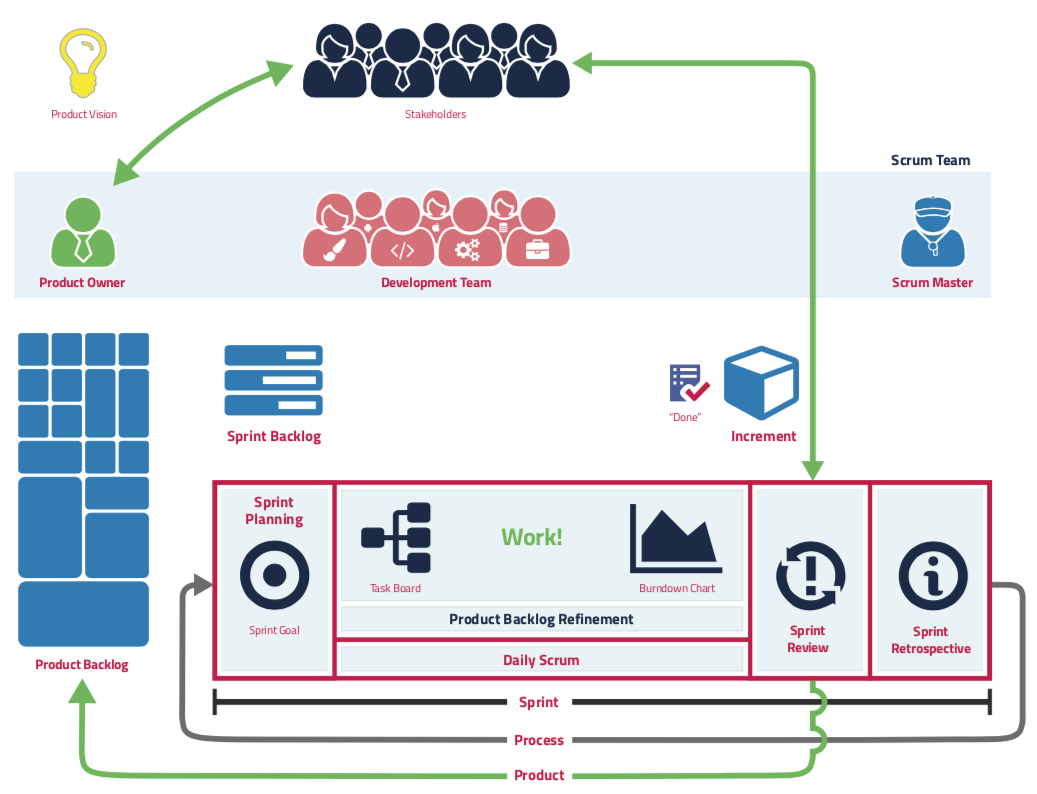
\includegraphics[width=\textwidth, height=100mm]
    {sdlc/scrum.png}
    \caption{The Scrum Workflow \cite{apd}}
    \label{fig:scrumworkflow}
\end{figure}

Scrum events took place such as sprint planning, daily scrum, review, retrospective, and backlog refinement. Sprint planning always took place on the first day of the sprint where three key indicators are outlined, what can get done in the sprint, how the work is done, and the sprint goal \cite{schwaber}, providing the development team an objective. This event usually lasts about one to two hours for a two week sprint. Due to careful planning at the start of every sprint, this led to successful sprints during implementation and being able to deliver on requirements.

Conducting daily scrum proved challenging from the beginning as members were not always on campus at the same time; to resolve this, stand-up would take place almost every two days, and at least four times a week. In both terms at the start of every lab, and every supervisor meeting a ten minute stand-up would happen in person. The other two meetings would happen virtually on \url{appear.in} for ten minutes, the day before a milestone deadline (Thursday), and either Saturday or Sunday - depending on the group's availability. Using this model allowed for quick decision-making, and removing any obstacles the team faced.

A sprint review took place to audit the work completed, the positives, negatives, and problems of the sprint. At this point, the group would decide if the tasks assigned were at a "done" status, subject to review of the product owner. All requirements that were outlined within a reasonable time constraint must be reached to achieve this status. If there are any outstanding tasks to be completed, then this would filter through to the following sprint planning, and the product backlog will be edited accordingly. This formed part of the sprint retrospective, but mainly focused on how well the team administered the methodology. Other key stakeholders are consulted here, giving any important feedback to the completed work.

The team used a scrum board in order to track tasks and make any changes during sprints. This promoted transparency amongst the group, and ensured accountability was retained. The project used other scrum artifacts discussed in chapter five. Overall, the execution of the Agile methodology was good, since two members of the team had worked together in projects using Agile in industry - leading to a greater understanding by everyone of how it works. However, during the first two sprints the scrum master was involved in the sprints themselves, and that lead to work not meeting requirements. This was rectified in the remaining sprints, where timely interventions at impediments took place by them so that momentum was conserved, and the outlined requirements were achieved.

\section{Test-Driven Development (TDD)}
Another development methodology used was TDD. Before completing implementation for the sprint, the unit tests were written so that the focus when writing source code is to make all the tests pass. This allows for the software architecture to be thought out beforehand, and ensure that the core functionality is acting on the requirements. Also, this methodology is proved to reduce defect density, and reduces cost since the testing time is dramatically reduced \cite{bulajic}. Further, TDD fits into Agile's iterative approach, providing ease of allocating resources in sprints, and all developers have a great understanding in this.

% Figure here
\begin{figure}[H]
    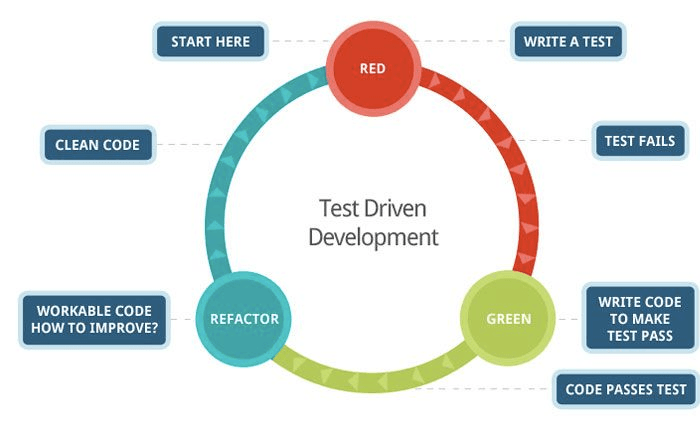
\includegraphics[width=\textwidth]
    {sdlc/tdd.png}
    \caption{The TDD Workflow \cite{k2datascience}}
    \label{fig:tddworkflow}
\end{figure}

Business-driven development, and acceptance test-driven development were considered, but a more thorough and rigorous testing system that focused mainly on the implementation was favored to deliver a working MVP.

% \section{Tools}

% @book{,
%     title     = {},
%     author    = {},
%     publisher = {},
%     year      = {}
% }

% @online{,
%     title     = {},
%     author 	= {},
%     url 		= {},
%     publisher = {},
%     year 		= {}
% }

% @article{,
%     author  	= {},
%     title   	= {},
%     journal 	= {},
%     year    	= {},
%     month   	= {},
%     pages   	= {},
%     url     	= {}
% }

% \add{}
% \remove{}
% \change{}{}
% \note{}

\chapter{Requirements}
\section{Stakeholders}
Nick Week 1

Stakeholders hold a very important position during a product's development; often influencing the outcome of a project by way of its scope, means of function and overall effectiveness and success. In foresight of this impact, we were keen to detect and appoint all appropriate audiences to this rank.

Fundamentally, the group at the centre is the \change{End User. In}{end users; in} In near-to-every circumstance, \note{not so keen on the hierarchy point here} if those at the bottom on any sort of hierarchy reject an idea or practice, those above will not benefit through its implementation. Furthermore, this is exacerbated as this project will largely change the \change{End User's}{end user's} experience of a museum which, \annote{if rejected by the that ilk}{rephrase this}, may lead to a decline in visits \remove{and, thereafter, in funding}. To understand our potential impact, we surveyed visitors and junior members of museum staff of the Science Museum and the Natural History Museum. 

Though this project was the product of an academic environment, it \change{isnt't}{is not} too unlike the real world in that we had we had direction set by this project’s supervisor, Dr. Basil Elmasri  and standards set by Dr. Nick Hine – the \remove{Group Project Module Leader}{module leader}. Given this project had to adhere to College's marking criteria, our supervisors responsibility was to ensure that we were at least doing so. Furthermore, the quality of work \remove{we would} produced would \remove{also} be representative of them. 

As this project is framed around being a main point of interaction between museums and visitors, it could affect the experience and potentially having an adverse effect. \annote{Because of this, we deemed it so, those in industry had a stake in this project. For us, 'those in industry' is two-fold: indoor navigation and creators of exhibits or those who know about the representation thereof.}{rephrase this} \annote{There has been a flurry of interest recently into indoor navigation across the technology sector. Given the excitement surrounding this,}{already mentioned in chapter 2} we were keen to get an experienced understanding. We were able to communicate with an incubator company, Pathfindr, via the Managing Director, Matt Isherwood. \note{what does pathfindr do} \remove{We see these experts as key stakeholders not only through our assassination, but as we are representatives for this growing chapter in computing.}

Seeking opinions from those in the business of being responsible for exhibits or creative works, we made it a priority of to gauge this stakeholder \annote{via online surveying}{change this to another interviewing method}. Getting the full scope of their opinion in relation to this project as our project will directly change how \change{the End User}{end users} interacts with the exhibit, leading to either hindering or bettering their experience. 

\annote{Finally, we, as the team behind this project, have a somewhat large stake in its success. Not only that if we didn't submit a quality report, but this new part of the technology sector may lose out on what we have, or would have, found.}{rephrase}
\note{need to mention who the project sponsor would be, or basil would be acting it basically}


\section{Gathering}
Nick Week 1

\note{planning to merge this with the user consultation section}
In presenting our System Requirements Specification (SRS) to our stakeholders, we were able to determine via our surveying their approval. Along with (cite stakeholder survey response) Feedback was positive and we were further encouraged by staff describing the current system of charging the current system of charging for maps and their current app solution as inadequate and cited often having to help visitors having simple issues navigating. We made it our business to visualise as much as possible the user experience to ease its otherwise, seemingly complicated description. Constructing the diagram showing our use case made it easy to demonstrate the project and, furthermore, inspired, jointly with our user requirements, the first graphical prototypes took shape. Using Adobe XD, we quickly made a mockup of the final design which allowed for a clear commination twix us and the stakeholders. 


\section{System}
Arif Week 1

\note{say what the system requirements are (i.e. describe what hardware/OS/middleware software should be run on.) and the justifications for that}
The SRS was designed to show the structured collection of the requirements of the system along with its operational environments, and external interfaces. The specification was written according to the ISO standard for systems and software engineering. The purpose, scope, and system overview serve to provide an outline of the overall platform. Use cases diagrams from chapter four are fully described in the specification.

% What is SRS?
A software requirement specification otherwise known as SRS is a description of a software system to be developed. SRS is used to layout the functional and non-functional requirements of a system. As well as that, a software requirement specification should include definitions of both system and user requirements, it should describe fully what the software will be. \note{These two paragraphs are basically the same, combine into one that makes sense.}

% {How we used it?}
Our system specification requirements clearly defines what type of software application we are going to be building. We used the SRS to know all the requirements for our application, which helped us in designing the software. \note{more detail needed}

% {why did we use SRS?}
\add{The} system specification requirements creates a bond between the \change{developers}{development team} and \change{clients,}{key stakeholders;} it allows them come to a conclusion about what \remove{should be implemented} and how it should be implemented. Without \change{a}{the} SRS it would be hard to know what needs doesn't need to be implement, also it creates a lot of \remove{mess and} confusion between \change{the clients and developers}{stakeholders}, and creates a mismatch of expectations. \remove{Which in the end is disadvantageous to both customer and developer.} \note{more reasoning needed here - look up online why the srs is good}

\section*{Constraints, Assumptions and Dependencies}
\begin{enumerate}
    \item \textbf{Internet Connection}: The application would not be able to query mapping services or have access to exhibit information otherwise.
    \item \textbf{Android}: Users of this application are Android device users that requires assistance in museum navigation. Devices that support basic dependencies of the application is expected for proper user experience.
    \item \textbf{ARCore enabled device}: users device must be compatible with ARCore for them to have access to the application's AR navigation.
\end{enumerate}


\section{Functional}
Arif Week 1

\note{moved this from the system requirements section}
\add{The functional requirements comprise of the system behaviour, the functions and features (what the system should do). It considers the key features such as the user navigation and its relative implications.}

\note{You need to go into more detail about each point, look at how you wrote the non-functional section, and check the essay plan}
\begin{enumerate}
	\item \textbf{}: Needs to be able to navigate the user from point A to B.
	\item \textbf{}: The system should be able to display navigational routes in real-time.
	\item \textbf{}: It should be able to calculate the quickest route.
	\item \textbf{}: A 3D line should be superimposed through augmented reality to display the navigation to the user’s destination.
	\item \textbf{}: Camera recognition on artwork/exhibits, displaying further information about the exhibit.
	\item \textbf{}: When user arrives at destination, the system should give a recommen- dation based on their route.
\end{enumerate}



\section{Non-Functional}
Arif Week 1

\note{moved this from the system requirements section}
\add{The non-functional requirements place constraints on how the system should do it. This considers the usability of the application, describing aspects such as performance, user actions, and safety.}
\begin{enumerate}
	\item \textbf{Performance}: The system should respond quickly to user input, e.g user wants to find more information about an art piece or whenever they search up a location. The system should not require extensive CPU usage, it should not slow the device down inconveniencing the user.
	\item \textbf{Usability}: The system should have a simple layout, with appropriate colour used in appropriate contexts. The language used on the app should be easy to understand for the users. Having done research based on the user preference, it was discovered that users dislike too much text on their menu screen.
	\item \textbf{Data Usage}: Data usage should be kept to a minimum, only querying the relevant information (user location and exhibit information). Also, the app would require internet connection in order to calculate the real- time distance of the final destination from the user’s current location.
	\item \textbf{Safety}: The system needs to have the ability to detect immutable objects obstructing the user’s path. This can reduce common user accidents when using a mobile phone whilst walking.
	\item \textbf{Security}: Ensuring that the device’s current location cannot be obtained by unauthorised third-party users is crucial in ensuing the security of using the platform.
\end{enumerate}


\chapter{Design}
\section{Models}
Gabe week 1

\subsection{Use Case}


\subsection{Activity}


\section{User Interface}
Hamza Week 1

The project lends substantial importance to its user interface and experience. As it will be used by people with a wide range of technical ability, the aim will be to make the app as simple as possible without having an impinging effect on any service the end product will feature. This prerequisite was clearly outlined in the surveying of museum guests and staff alike. The first mission was determining what interfaces, and experiences currently exists within the museum sector. Many museums employed simple interfaces but due to their mass-manufacturing, their design felt unoptimised with simple bare-bones media not beyond text and images. Furthermore, this design would fail to deliver anything more complex than texts and images.
  
The approach to the UI/UX prototyping was to create different interface mock ups and exhibit them alongside existing solutions. An initial storyboard was drawn up and three potential interfaces (Figure~\ref{fig:prototype1}~\ref{fig:prototype2}~\ref{fig:prototype3}) were designed and shown to stakeholders. The feedback gained from the stakeholders was invaluable in the process as it allowed for the group to \change{understand the positive and negative attributes}{consider all aspects} of the prototypes. It was decided that a final version of the application's user interface would be designed, implementing all the positive attributes, and combining it into one (Figure~\ref{fig:finaloverview}), whilst also considering the negative attributes.

Figure here

% \subsubsection{Prototype 1}
% \begin{figure}[H]
%     \centering
%     \includegraphics[width=\textwidth]
%     {prototypes/ui/1.png}
%     \caption{Overview of UI Prototype 1}
%     \label{fig:prototype1}
% \end{figure}

% \subsubsection{Prototype 2}
% \begin{figure}[H]
%     \centering
%     \includegraphics[width=\textwidth]
%     {prototypes/ui/2.png}
%     \caption{Overview of UI Prototype 2}
%     \label{fig:prototype2}
% \end{figure}

% \subsubsection{Prototype 3}
% \begin{figure}[H]
%     \centering
%     \includegraphics[width=\textwidth]
%     {prototypes/ui/3.png}
%     \caption{Overview of UI Prototype 3}
%     \label{fig:prototype3}
% \end{figure}

\newpage

Figure here
% \subsubsection{Final Prototype}
% \begin{figure}[H]
%     \centering
%     \includegraphics[angle=90, width=\textwidth]
%     {prototypes/ui/final.png}
%     \caption{Overview of final UI prototype}
%     \label{fig:finaloverview}
% \end{figure}

\newpage


\section{Technical Architecture}
Gabe Week 1

\section{Accessibility}
Arif Week 1

Accessibility is about making \change{your application usable}{the product} to majority of \change{your audience}{end users}. \change{Our Application}{The application} provides accessibility as part of the service we are offering to our audience and a way to make our app more generally appealing. Some accessibility options would include features such as relating to mobility, colour perception, \add{and} literacy \remove{etc}.

\begin{enumerate}
	\item \textbf{Screen Reading}: \remove{Screen reading is one of features which we have used in our app.} Users tend to rely on a screen reader to help them interact with the app, \change{therefore our app includes}{including} UI elements, such as name, role, description, state and value. This feature would allow the user to use the app without any difficulties since the layout is simple and straightforward. 

	\item \textbf{Keyboard Accessibility}: This accessibility feature would allow users to interact with all UI elements within the application by keyboard only. It enables users to navigate through the app by using arrow keys. Allows the users to activate UI elements in the app by using Enter keys. Allows the users to enter their current and final location using the keyword. \note{This one is too bullet pointy - can you make it more prose like so it flows better?}

	\item \textbf{Scale}: \note{Don't use first person} We used scale to allow users to zoom and resize some elements, our main thought behind this was to help people with visual impairment, especially for images that include words. We also made sure to not start with a font size that is too small in general for many users, the reason behind this was because everyone’s vision deteriorates as they age; and we wanted to make sure our app is usable for users of any age. \remove{That's all that we have been able to get done so far, however}\add{In future iterations}, we are thinking of allowing differences in vision, the way we are doing this will be by providing different scaling options for our users in the app settings. This means they can change the font size for easier reading or even shrink or enlarge the UI as well for better vision. \note{talk about how scale affects the augmented reality part, and how to avoid motion sickness}

	\item \textbf{Vision}: The text and UI in \change{our}{the} app is designed to support high-contrast theme. \remove{We know that} \change{while}{Whilst} colour is important, it must not be the only channel of communicating information. For instance, users who are colour blind would not be able to distinguish some colour status indicators from their surroundings. Therefore \change{we have included}{,} other visual cues such as text \add{are included} in order to ensure the on the app information is accessible to everyone. 
    
\end{enumerate}

\section{User consultations}
Hamza Week 1

\note{Might convert this section to requirements gathering}
\remove{Consultation addressed potential} \add{End-}users and other key stakeholders such as an interested domain expert, Matt Isherwood, Managing Director at Fuse\textsuperscript{\textcopyright}, \add{were consulted during the design stage} to clarify \change{their}{user} needs and requirements. In addition to our \remove{online questionnaires and } online interactions with our stakeholders, the group had also conducted field research, and had face-to-face talks with potential users at \change{museums in London (e.g.} the Natural History Museum, Science Museum, \add{and} the V\&A museum \remove{)} to obtain \add{a} more nuanced input from key stakeholders. When prototyping the application, drawing and designing the user interface was not as simple as bringing ideas to life - it was imperative that our users were consulted when making these decisions. 

Upon consulting the users, it became apparently easier to actualize the designs put forward - acknowledging the fact that the users had all required a system that was relatively simple to navigate around. However, users were also consulted when it came to the technical aspect of the project. For example, deciding which medium would be best to track user location was one of the questions that arised in the early stages of development. \add{In that regard,} \remove{consulted} Mr Isherwood \add{was consulted} about this, and he \remove{had} brought to light the plethora of solutions that were readily available to begin development, primarily highlighting that the use of \change{bluetooth}{Bluetooth} beacons would be most efficient to implement given the scope of the project. \note{Why did Matt say Bluetooth was good?} \note{Add somewhere we spoke to some Fine Art students at the University of Oxford to give us perspective on user experience etc.}

\chapter{Implementation}
\section{Backlog}
\begin{figure}[H]
    \centering
    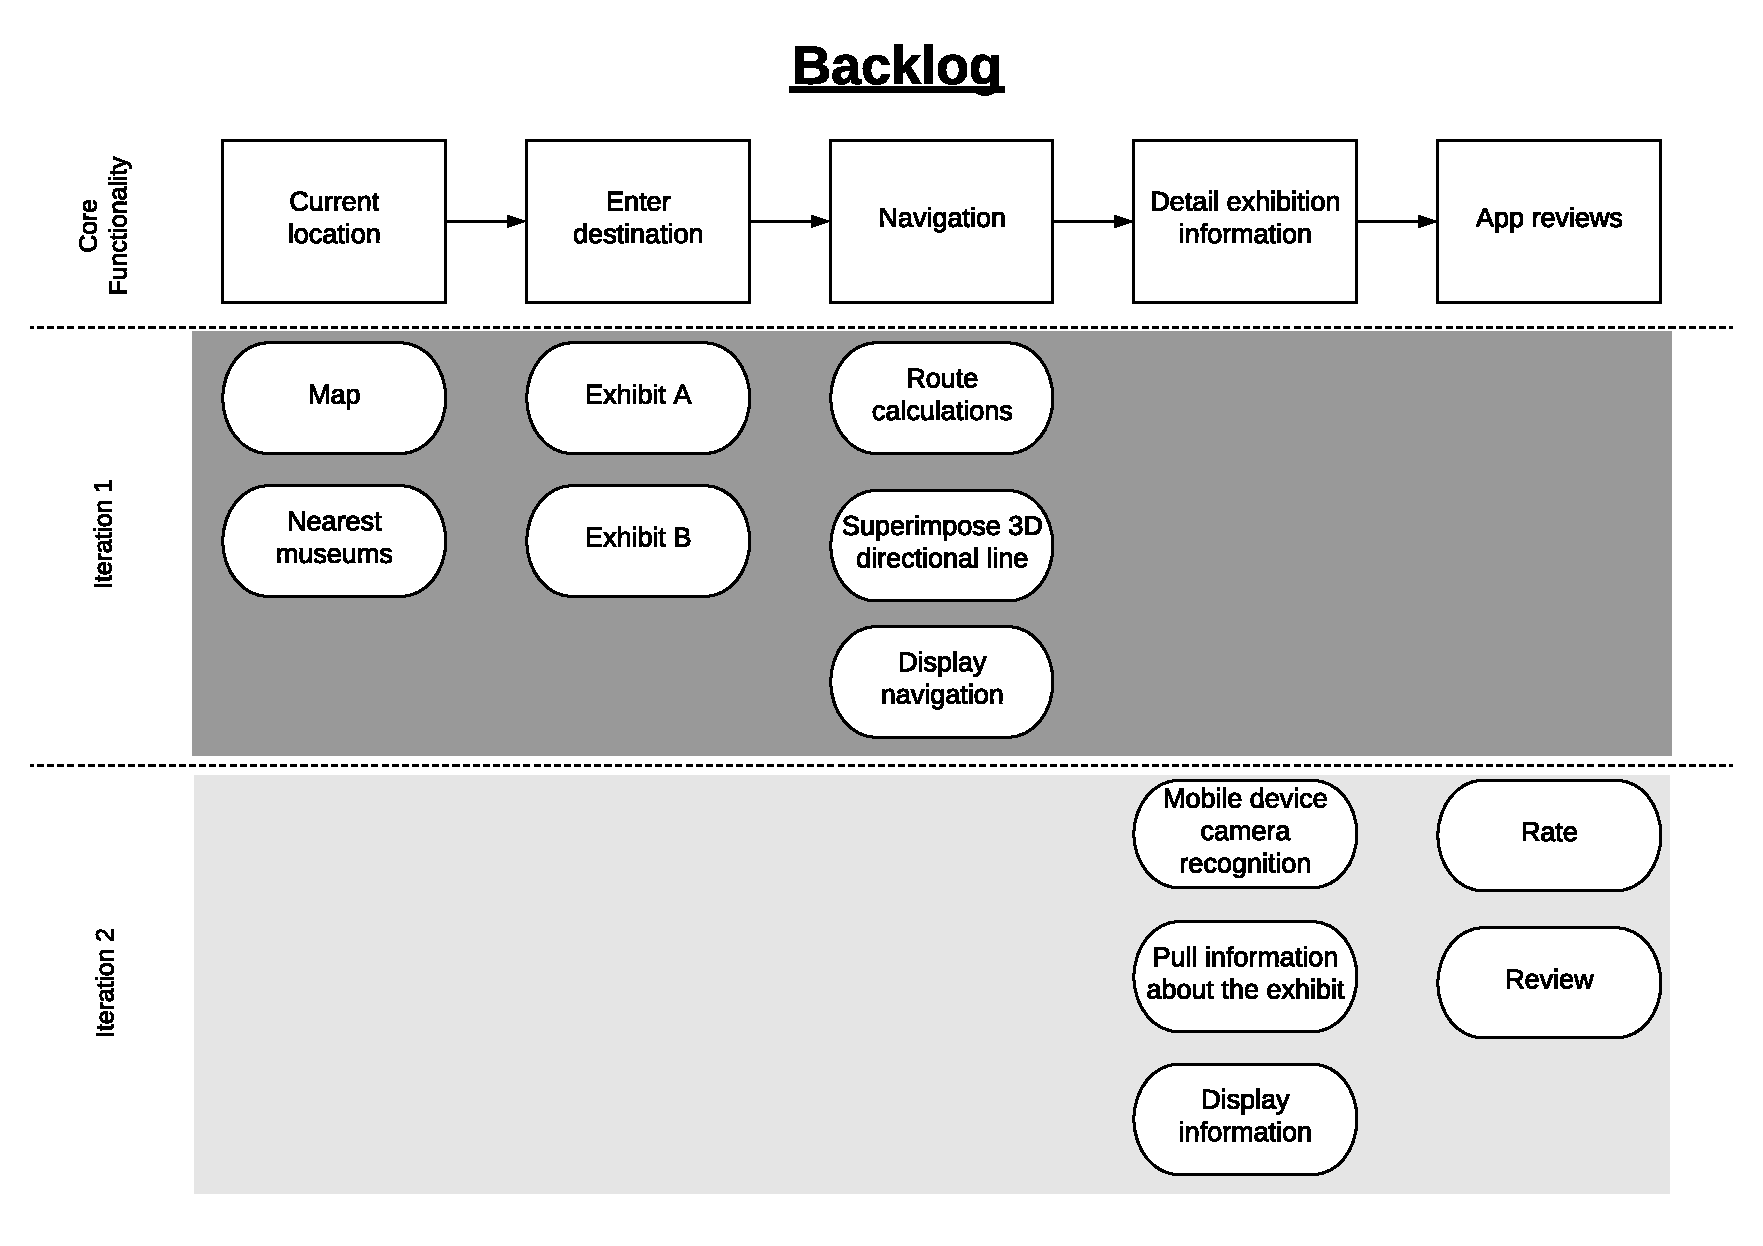
\includegraphics[width=\textwidth]
    {technicalarchitecture/backlog.pdf}
    \caption{Inital Product Backlog}
    \label{fig:productbacklog}
\end{figure}

The product backlog was used as the single source of requirements in order to prioritise releases, and allowed for transparent iteration planning. From the requirements and project scope, each of the five core functionalities were broken down into its major components. Considering the time estimates, the scrum team decided that to demonstrate originality in the project, and to build the base functionalities first, the route calculations and the AR implementation were to form the MVP. Features which required a database such as exhibition item/image recognition, user profiles/logins, and building servers were placed in future releases. These components would take longer than the amount of development time available along with the base functionalities. The team recognised the added time for the construction and integration of a database to the app would increase the risk in not delivering a functional MVP. As a living scrum artifact, the backlog changed accordingly when there were requirements, enhancements, and fixes during the implementation and testing phases of each sprint. In practice, the backlog was maintained on the scrum board hosted on Trello.

% table of time estimates
\begingroup
\renewcommand{\arraystretch}{1.5} % Default value: 1
\begin{table}[H]
\centering
\begin{tabular}{l|c}
\textbf{Function}                & \textbf{Estimate Time (Days)} \\ \hline
Displaying map                   & 0.5                           \\
Finding nearest museums          & 3                             \\
Getting start and end locations  & 5                             \\
Route calculations               & 10                            \\
Superimpose 3D directional line  & 12                            \\
Displaying navigation            & 10                            \\
Mobile device camera recognition & 2                             \\
Retrieve exhibit information     & 10                            \\
Display exhibit information      & 1                             \\
Rating the app                   & 1                             \\
Reviewing the museum visit       & 3                             
\end{tabular}
\caption{Table of time estimates for each function}
\label{table:timeestimates}
\end{table}
\endgroup

\begin{figure}[H]
    \includegraphics[width=\textwidth, height=100mm]
    {sdlc/scrumboard.png}
    \caption{Snapshot of scrum board in action}
    \label{fig:scrumboard}
\end{figure}

\section{Sprint Outlines}
During implementation, four sprints were conducted each lasting one to two weeks. The first sprint lasting one week with the goal of building a beacon for calculating distances between users and objects. The following sprint focused on route calculations; being able to calculate the route between two points in a given space. For the AR part, this was divided into two separate sprints, with the initial one focusing on rendering, and anchoring objects in real-time, and afterwards the integration with all base functionalities.

\section{Front-end}
Front-end development was carried out using Java on Android Studio. 

It was carried out in the early stages of implementation due to the fact that the team had already received user feedback for the UI/UX prototypes. After combining the positive features of the initial design prototypes into one, it became easier to visualise the end result. With aims to create an user interface that is user friendly, and intuitive, various features of the application are self-explanatory. 

As soon as the application is opened, the user is faced with the login page asking for credentials. The user can keep track of their past visits to museums and review various sites; this put in place future developments but not included in the MVP. However, if the user does not have an account they are able to 'Continue as a Guest', and use the services freely without saving any data. When the user has passed the login page, they see the menu.

\begin{figure}[H]
    \centering
    \begin{minipage}[b]{0.4\textwidth}
        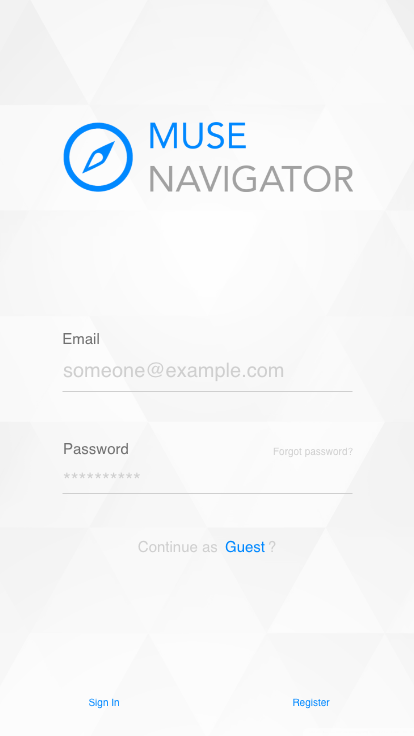
\includegraphics[width=50mm]{prototypes/ui/final/1.png}
        \caption{Log-In Screen}
        \label{fig:loginscreen}
    \end{minipage}
    \qquad
    \begin{minipage}[b]{0.4\textwidth}
        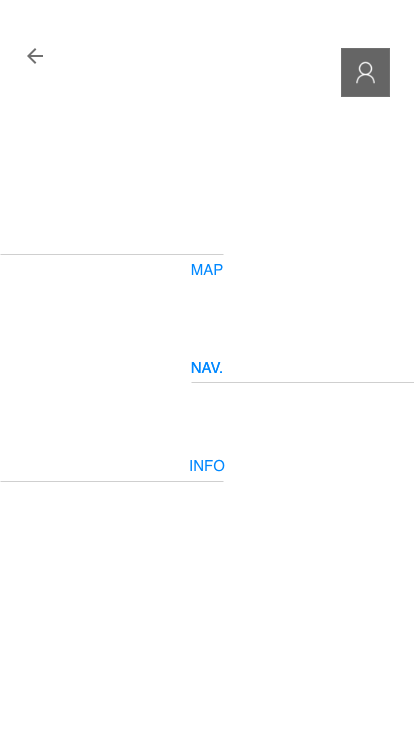
\includegraphics[width=50mm]{prototypes/ui/final/2.png}
        \caption{Menu Screen}
        \label{fig:menuscreen}
    \end{minipage}
\end{figure}

There are three different services that the user can utilise. The 'Map' which shows the user their current location, and surroundings on a 2D map. The 'Nav' menu takes the user to the screen which the user has to then enter their desired destination or exhibit. After all the information has been entered by the user, the user's device displays the AR-enabled camera with the highlighted navigational line directing the user to their destination. However, if the user's device is not compatible with Google's ARCore then the user will not see this screen, and instead faced with an error message. Lastly, the 'info' page will allow the user to see additional information about an exhibit of their choice - this also requires the user to fill out a form.

\lstinputlisting[language=Java, firstline=46, lastline=71]{src/MenuActivity.java}

\begin{figure}[H]
    \centering
    \begin{minipage}[b]{0.4\textwidth}
        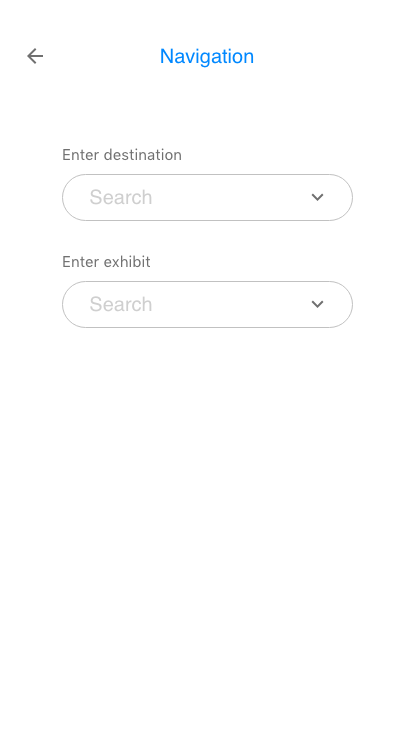
\includegraphics[width=50mm]{prototypes/ui/final/6a.png}
        \caption{Enter Destination}
        \label{fig:enterdestination}
    \end{minipage}
    \qquad
    \begin{minipage}[b]{0.4\textwidth}
        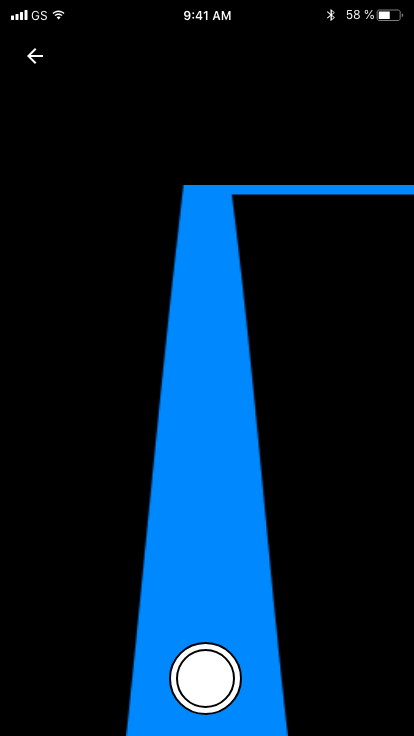
\includegraphics[width=50mm]{prototypes/ui/final/7.png}
        \caption{Navigation Screen}
        \label{fig:navscreen}
    \end{minipage}
\end{figure}

As a result of all the planning and prototyping, when it came to actualising the design in Android Studio it was as simple as writing code for implementation - no further designing was needed, with exception of minor changes such as font sizes.

\begin{figure}[H]
    \centering
    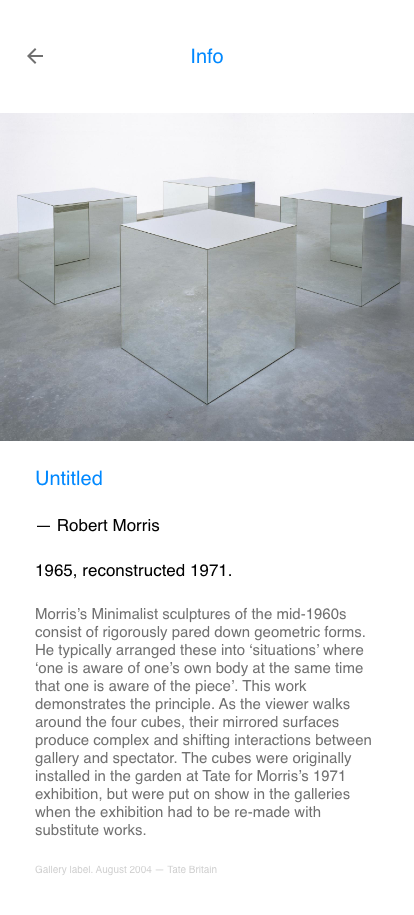
\includegraphics[width=50mm]
    {prototypes/ui/final/8.png}
    \caption{Additional information}
    \label{fig:infoscreen}
\end{figure}

\section{Back-end}
The back-end implementation consisted of developing the application's AR, and route calculations systems, along with integrating, and testing the two constantly throughout the process.

\subsection{Route Calculations}
The scrum team delegated both a sprint, and a consultation with the domain expert in order to ensure this was done correctly.

This concluded in the route calculations using the A* path finding algorithm. Bluetooth was an option in development however, the errors that Bluetooth navigation provided were difficult to handle. Also, the A* algorithm is a better fit for the back-end, since they are both complimentary to augmented reality.

Developed in Kotlin (for development speed), and then converted to Java (to be integrated with the AR segment), the user first enters a destination. That destination becomes a goal node in the context of the route calculations. An attempt to calculate the shortest route using a graph, then outputs that route via the 3D line. As the user traverses that line, their location is constantly updated relative to the goal node so that when the user reaches it, and an alert is shown. It also ensures that the path constantly updates in the case that they ever lose their way.

\subsection{Augmented Reality}
The application's AR research began with the group understanding how Android's ARCore operates with the camera. It was found that the library evaluates the camera's pixels as a set of 2D nodes - it then maps those 2D nodes onto a 3D plane using depth perception \cite{}. This meant that in order to superimpose the 3D line. The output of the route calculations would have to have little, to negligible margin for error. Otherwise, the user could be guided incorrectly.

Once the research was completed, the group delegated a sprint and some research time beforehand to setting up the AR environment that would be utilised by the route calculation system. Therefore, over the sprint, a testing plan was formulated with seven tests to ensure the environment worked in a sound fashion.

\lstinputlisting[language=Java, firstline=93, lastline=115, caption=Creating AR Scene]{src/ARActivity.java}

The AR sceneform (which assists in rendering straightforward 3D scenes without OpenGL) is retreived from the UX XML fragment and the AR Activity fragment. THe model is then setup and rendered with an sfb file (the line), and if unrenderable, an exception is thrown. Using the device's camera, when a flat surface is recognised, the object's position is anchored on the device's screen. After, transformable functions are added to the line including qualities such as scale, and position. Finally, the line is then displayed.

\lstinputlisting[language=Java, firstline=118, lastline=127, caption=Setup Model]{src/ARActivity.java}
\lstinputlisting[language=Java, firstline=129, lastline=134, caption=Creating Model]{src/ARActivity.java}

\begin{figure}[H]
    \centering
    \begin{minipage}[b]{0.4\textwidth}
        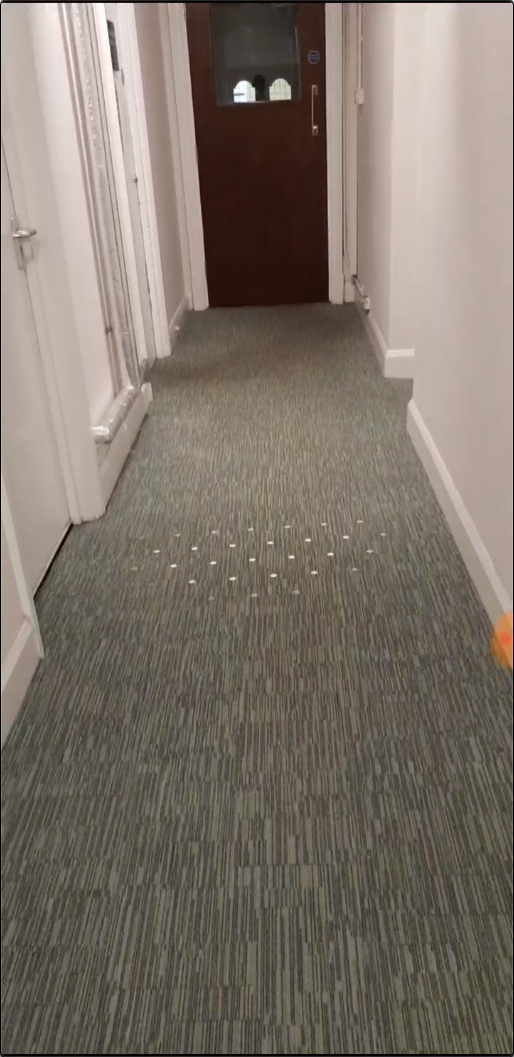
\includegraphics[width=50mm]{final/ar1.png}
        \caption{Detecting flat surface}
        \label{fig:flatsurface}
    \end{minipage}
    \qquad
    \begin{minipage}[b]{0.4\textwidth}
        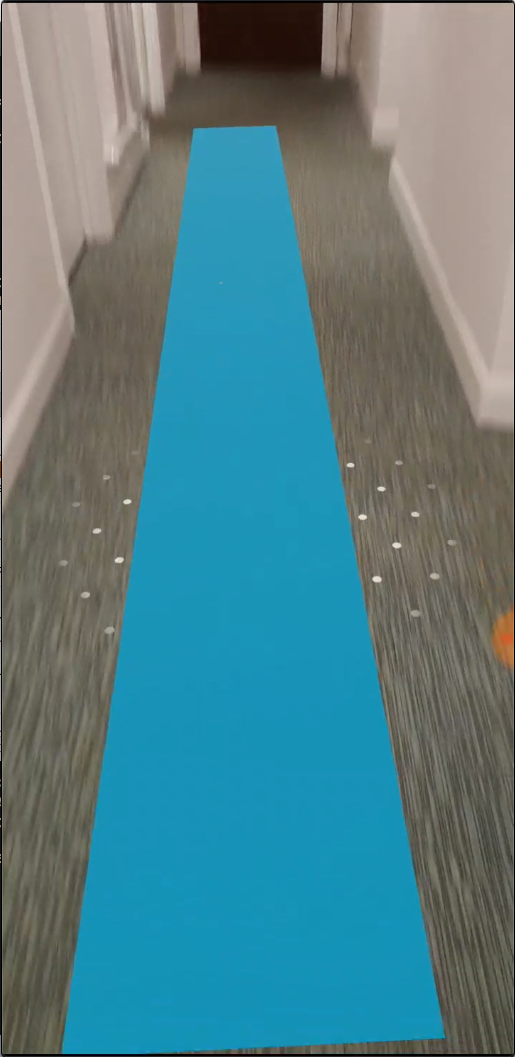
\includegraphics[width=50mm]{final/ar2.png}
        \caption{Anchoring, and displaying straight line object}
        \label{fig:anchor}
    \end{minipage}
\end{figure}

\section{Hardware}
In order to transmit the user’s location to compute a route solution, utilising the Arduino (UNO R3 Mega 2560)’s small foot-print, a simple beacon plan was sought consisting of the Arduino coupled with the Bluetooth HC- 05 RF transceiver. 
 
Figure~\ref{fig:arduino} displays the basic layout of the beacon aside from power input via the board’s USB-B socket. This configuration was able to send the strength of the Bluetooth frequency thereby allowing the computation of a distance.

\begin{figure}[H]
    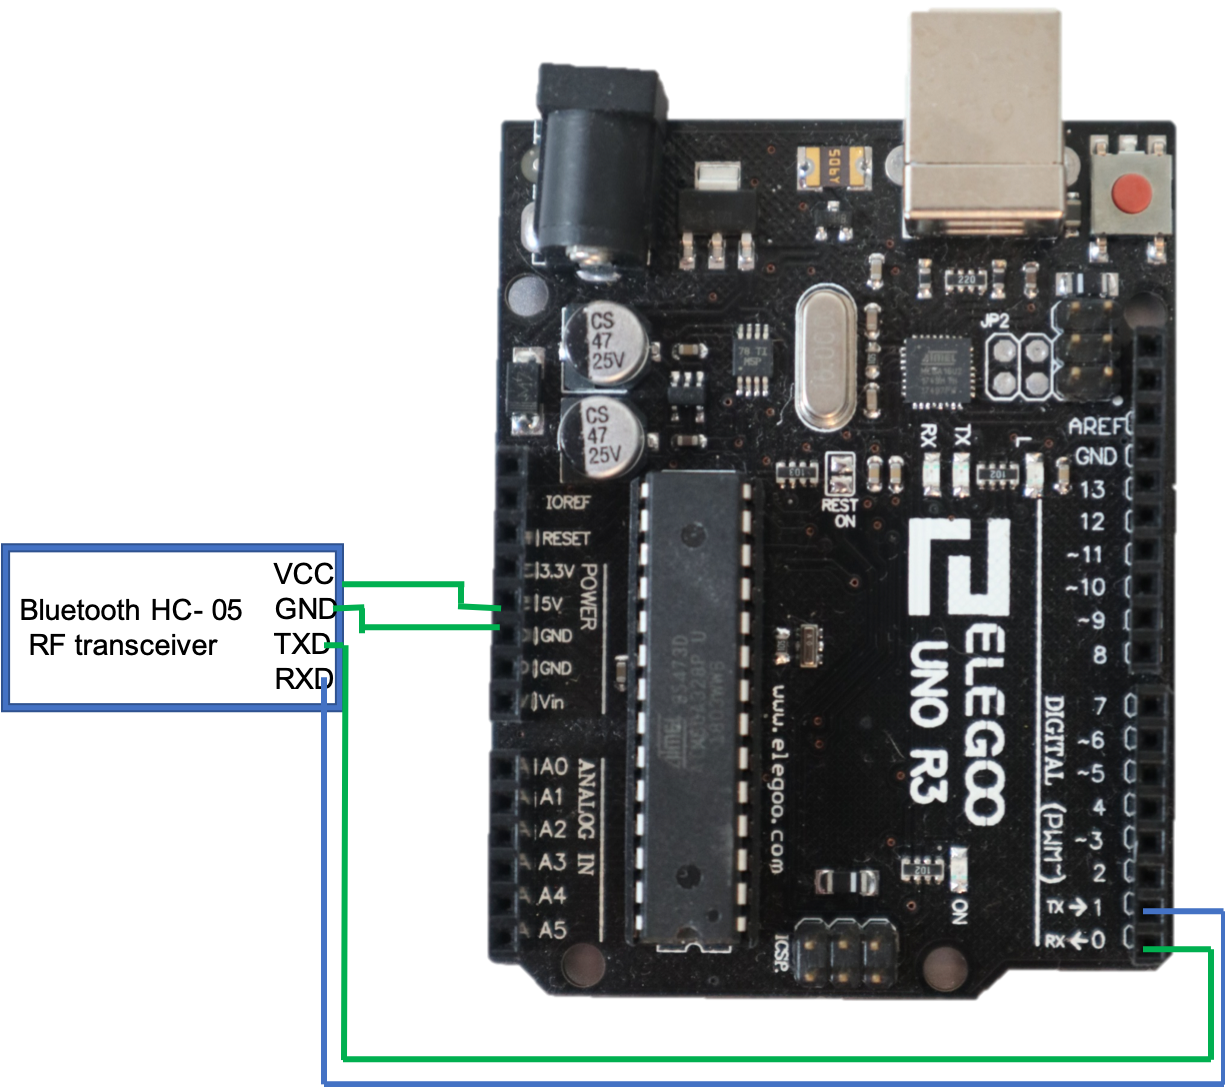
\includegraphics[width=\textwidth, height=100mm]
    {arduino/arduino.png}
    \caption{Arduino layout}
    \label{fig:arduino}
\end{figure}

However, to get more accurate readings, the project would need at least three beacons to demonstrate triangulation wherein three signals are emitted from three angles to get an accurate location. During the testing there was only sufficient means for the procurement of one beacon – this led to an inability to fairly showcase the ideal usage, hindering the projects in this method. 

While it was advised by the domain expert that this Bluetooth solution would be the best policy, it was not practicable given the available resources. In view of these drawbacks, the hardware proposal was ceased. The research provided the team with enough of the methods, and models to pursue a theoretical solution. 

\section{Ethical Audit}
To comply with GDPR, user locations are recorded during the runtime of the application, and upon termination this data is deleted from memory in order to prevent unauthoried access to the user's location. Users are asked initially to give the Bluetooth, camera, and location permissions to use particular functions.

Since the app uses museum maps, and exhibition details, the intellectual property for those will not be under the jurisdiction of the team. Rather, the project members owns the intellectual properties of all technologies that are being created, and used in conjunction with third-party information. Since assigning data and storing details to specific users was not implemented in this iteration, in future versions the app will need to prevent attacks such as SQL injections.

\section{Challenges}
The groups ideas were difficult to manifest due to a lack of technological resources, and a much larger, but relevant issue; the infancy of the AR, and accurate indoor navigation market-places.

Currently, the market relies on Bluetooth technology in order to bypass the problem. However, for this application, using Bluetooth has disadvantages that can prove crucial success to the project. First, the group would have to have access to multiple Arduinos in order to propagate the necessary number of Bluetooth RSSI signals to get an accurate position on the user. Without enough Arduinos, the group would be at risk evaluating the signals inaccurately due to the compromising of the signals by metallic surfaces. Another issue with the Bluetooth technology is the risk that it places the user in. 

The group initialised the solution by finding a prototype that had already existed \cite{smd}. Once found, another challenge arose; the prototype was last maintained in 2016 so the code did not function to begin with. This hurdle was solved by delegating a sprint to the debugging the application.

This halted the software development of the application for a period of time, until the prevailing solution had been devised. A theoretical solution would involve the group hard-coding the geometry of the area to be traversed by the user, and using the coded geospace along with a hard-coded location anchor within that geospace to navigate (A* algorithm with a vector function as the heuristic) the users device.

Finding problems with ARCore library, the group had problems debugging since documentation was vague and information was scarce. An example of a faced issue was the inability to have the AR section of the application open up on different mobile devices.

A large amount of implementation time was finding usable AR resources, namely the straight line to direct users. Initially, the line file was created, and rendered but did not display on the user's device. To resolve this, a different object file from a GitHub repository was utilised instead. In this case, the line was displayed on the screen, and the group came to resolve that it was an issue to do with the object file, and not sections of the source code.

Further, members of the development team had varying Android versions and SDKs during development, providing inconsistent experiences for each developer. Instead, more pair programming took place so instead of working in an ad-hoc fashion, a collaborative approach was used instead.

\chapter{Testing \& Quality Assurance}
\section{Testing conducted}


\subsection{Unit Testing}


\subsection{Integration Testing}


\subsection{Performance and stress testing}


\subsection{Regression testing}


\subsection{User Acceptance Testing (UAT)}


\subsection{Beta Testing}


\section{Deployment}


\section{Formative evaluation}


\section{Functional requirements review}


\section{Non-Functional requirements review}

\chapter{Project Evaluation}
\section{Summative Evaluation}
This project aimed to tackle indoor navigation in commercial settings specifically museums. Augmented reality was selected in order to enhance this, providing greater a user experience. Stakeholder gathering was valuable since it gave insight to problems the group did not foresee, and laid out the foundational requirements of the system. The execution of the Agile methodology was good, since two members of the team had worked together in projects using Agile in industry - leading to a greater understanding by everyone of how it works. 

Although most stakeholders had Android devices, more extensive research could have taken place on iOS since the team faced various problems regarding the Android operating system. Situations like Bluetooth signals being received by Apple instead of Android devices, and in contrast to Android, Apple offers thorough AR-related documentation which was realised during later stages.

Strong planning across the project was the key to success as all of the team contributed to tasks, allowing for leeway if issues arose. When team members were indisposed for example, re-allocating responsibilities were managed, and controlled the risk of overusing resources. Using Trello ensured responsibility was held to account, and centralised project management. Especially during the design stage of the project, this ensured that ideas were communicated across clearly to stakeholders. Since many Lo-fi prototypes were created, finding positive attributes to form the final design was straightforward as stakeholders were not limited in choice. 

Initially, finding one similar prototype for navigation assured Bluetooth was not the technology to use in calculating routes. The project sponsor informed that metal surfaces interferes with RSSI \cite{apple}, this lead to using path finding algorithms (in the context of graphs) instead as AR better supports it. During the first two sprints the scrum master was involved in the sprints themselves, and that lead to work not meeting requirements. This was rectified in the remaining sprints, where timely interventions at impediments took place by them so that momentum was conserved, and the outlined requirements were achieved.

The decision by the team to control the scope of the MVP ensured that requirements were met within the timeframe. Sections of the app written in Kotlin were converted to Java in the final sprint since Android Studio better supports it. Further, more members were confident with Java, allowing for team members to rigorously test features, and finding resolutions. Controlling the scope allowed the demonstration of originality in this project, and provided discipline to adhere to the MVP; reducing risk in resources enabled for correctly implemented features in the app.

If given more time, further research could have been conducted into various technologies for calculating routes in the context of AR. At the start of the project lifecycle, academic research in the field has been relatively limited given its infancy, but has recently accelerated with large technology companies rolling out beta versions of outdoor AR navigation. Hence during the research stage, a greater understanding of the sector dynamics would benefit outlining requirements, and features to build for the MVP.

\section{Future Developments}
By design, this project is geared towards to meeting the requirement of the museum sector. However, the main objective navigation, being so widely applicable, with adequate research there are many prudent areas of development. With the saturation of navigation software, this project should strive to stick to the indoor avenue. 

In a commercial context the most important future development would be retail navigation. As the product is based on finding the shortest route to a point, taking the project to this stage would not require any fundamental change. As in this concept, a retail version would involve finding the best solution in terms of pure navigation, and also proposing certain shops in keeping with the user’s preferences should be made clear that based on the current model which involves studying the layout of a candidate area, a need to find a quicker method of digitising a space is desirable. 

Areas covered in the project backlog with the remaining features left to implement to create a fully working product would be an area of future development. Building a database to house previous user visits can further enhance the user experience. A more streamlined method of implementing individual floor plans would provide quicker lead times to potential clients in developing prototypes for their buildings, though this would be further down the line.

In addition, there is a plethora of other environments to explore. For instance, the findings of this report can be easily implemented into public libraries wherein you have a catalogue system for which the project could apply a node to which to navigate to. Furthermore, as most library users will look for a general subject or even a very specific book criteria, the efficiency of this project would be very well employed in bringing about unambiguous results and pathway. Other areas can also be exploited where there is a sense of urgency to reach a destination like airports or train stations whereby there is usually an abundance of space only supported by signposts to guide the way. The implementation of the project could have a positive impact in helping users quickly finding a pathway.


\afterpage{\blankpage}

%-----------------------
% APPENDICES
%-----------------------
\begin{appendices}

\chapter{User \& Stakeholder Research}
Nick Week 1

\note{um where's this?}

\chapter{User Stories}
\section*{Use Case Model}
Two scenarios have been taken into account, where the user gets lost in the museum, and the user wants to explore the museum. When a user is lost, they need to enter their destination where the app will receive their current location, and find the quickest route from the user's current position. The user follows that navigation until they arrive at their destination. For the exploration, the app will show the details where user know what they going to see in the museum.

\subsection*{Activity Model}
This is based on the back-end of the application for example when the user searches about the museum, this history saved in the server where if the user wants to go to the same place then they can use our function called past visit.

\section*{User \& Acceptance Stories}
This will describe what will be achieved once the application is ready to be used by the user. A diagram has been created based on different scenarios where it can be found if the application has achieved the user needs. 

\begin{figure}[H]
    \centering
    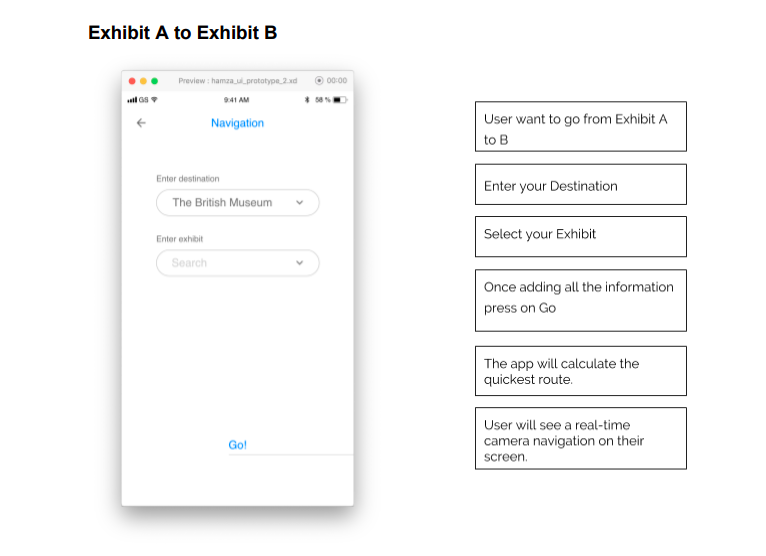
\includegraphics[width=\textwidth]
    {userstories/userstory_aTob.png}
    \caption{Going from point A to point B}
    \label{fig:AtoB}
\end{figure}

\begin{figure}[H]
    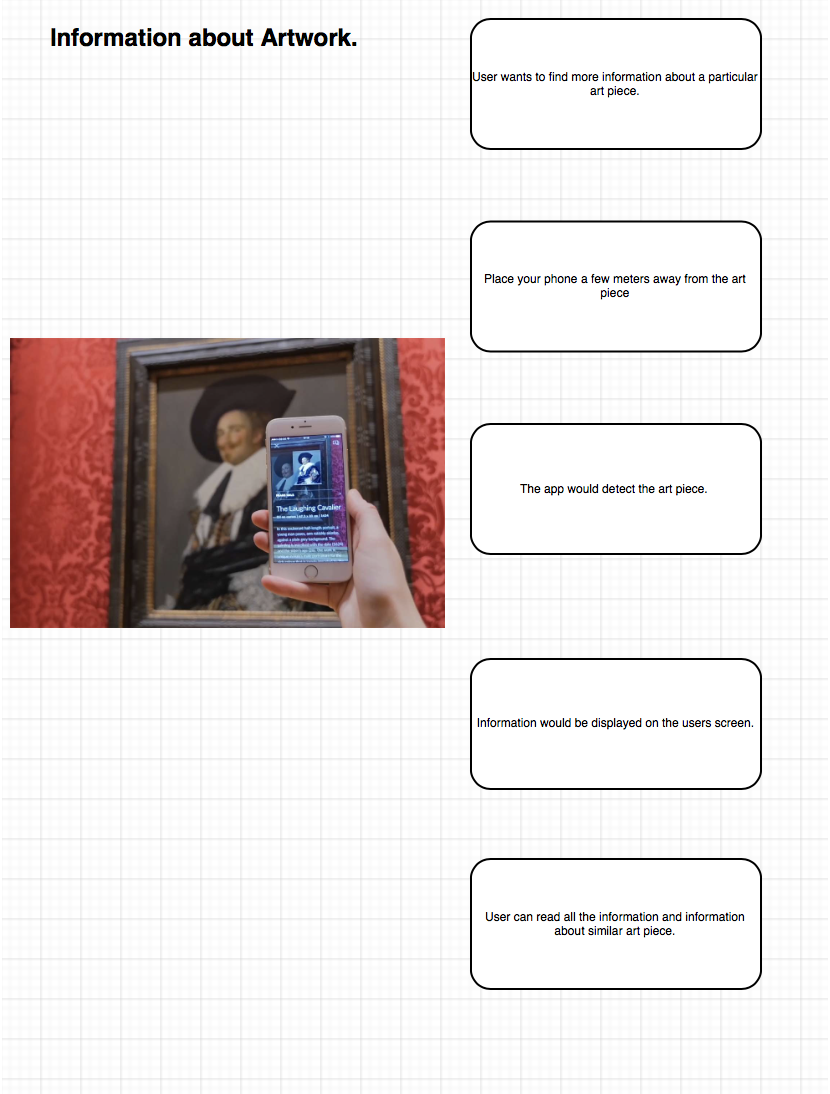
\includegraphics[width=\textwidth]
    {userstories/userstory_info.png}
    \caption{Getting information from exhibition}
    \label{fig:infofromexhibit}
\end{figure}

\begin{figure}[H]
    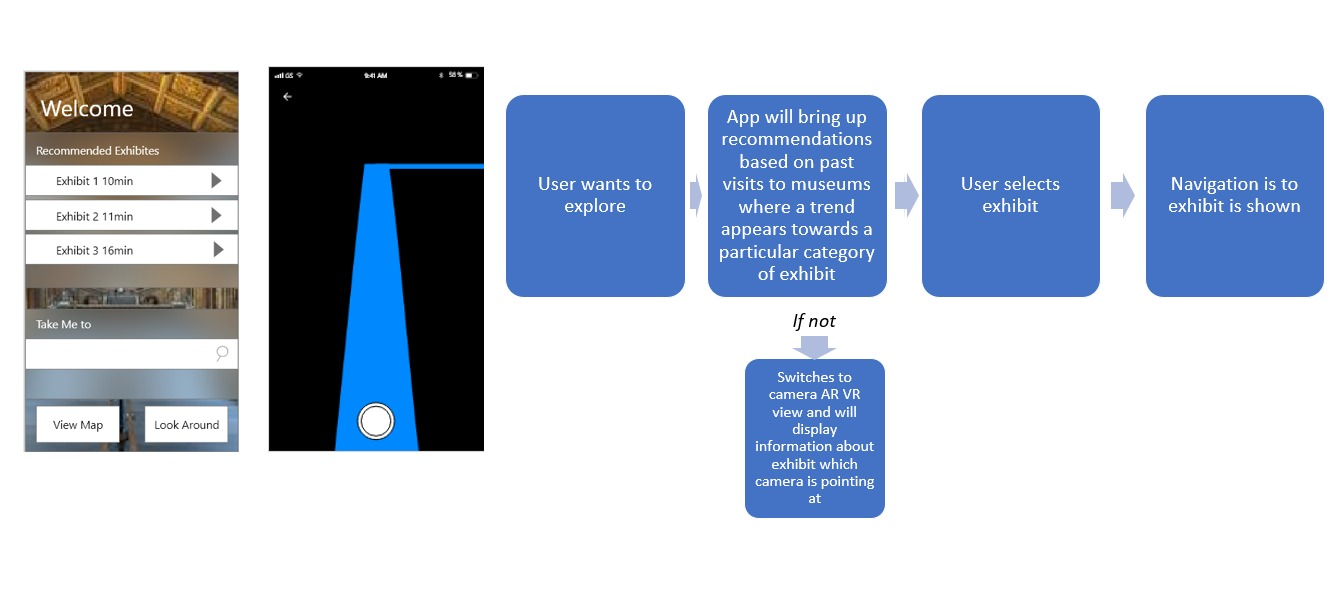
\includegraphics[width=\textwidth]
    {userstories/userstory_explore.jpeg}
    \caption{Exploring the museum}
    \label{fig:exploring}
\end{figure}


\chapter{Systems Requirements Specification}
\section*{Purpose}
The main goal of this concept is to provide users a solution to indoor museum navigation through an exciting, and enjoyable experience using augmented reality. It includes users being lost, or searching for a specific location within the museum. It was discovered through field research that the concept would make life easier for users and the museums since it would allow easy access to the information based on exhibitions.

\section*{Scope}
This project will include creating an AR application for people to get an enjoyable journey in the museum. The project will be completed by 29 April 2019. The AR application will include simple navigation system to direct various part of the museum. Getting information on the user screen using the user's camera, and explore various museum using the system. The platform will be developed on Android due to the high usage of Google's AR library, ARCore.

\section*{System Overview}
The application will perform all the basic tasks to help users with their journey in the museum. Such as navigating from point A to B, getting the user back on track in case they are lost, allowing the user to view information based on camera recognition of an exhibit.

\section*{References}
This specification should be read in conjunction with the following publications:

IEEE 24765-2017 - ISO/IEC/IEEE International Standard - Systems and software engineering--Vocabulary \cite{IEEE24765}

IEEE Std 29148-2011, ISO/IEC/IEEE International Standard - Systems and software engineering -- Life cycle processes --Requirements engineering \cite{IEEE29148} 

IEEE Std 730-2014, IEEE Standard for Software Quality Assurance Processes \cite{IEEE730} 

IEEE Std 24748-4-2016 - ISO/IEC/IEEE International Standard for Systems and Software Engineering -- Life Cycle Management -- Part 4: Systems Engineering Planning \cite{IEEE24748}

\section*{Definitions}
\textbf{Activity:} A set of cohesive tasks of a process, which transforms inputs into outputs. [ISO/IEC/IEEE 12207:2008]

\textbf{Augmented reality:} A technology that superimposes a computer-generated image on a user's view of the real world, thus providing a composite view.

\textbf{Functional requirement:} A requirement that specifies a function that a system or system component must perform. [ISO/IEC/IEEE 24765:2010]

\textbf{Non-functional requirement:} The measurable criterion that identifies a quality attribute of a function or how well a functional requirement must be accomplished. A non-functional requirement is always an attribute of a functional requirement. [ISO/IEC/IEEE 730:2014]

\textbf{Performance:} Degree to which a system or component accomplishes its designated functions within given constraints, such as speed, accuracy, or memory usage. [ISO/IEC/IEEE 24765:2017]

\textbf{Stakeholder:} Individual or organization having a right, share, claim or interest in a system or in its possession of characteristics that meet their need and expectations. [ISO/IEC/IEEE 15288:2015]

\textbf{Usability:} Extent to which a system, product or service can be used by specified users to achieve specified goals with effectiveness, efficiency and satisfaction in a specified context of use. [ISO/IEC/IEEE 25064:2013]

\textbf{User:} Individual or group that interacts with a system or benefits from a system during its utilisation. [ISO/IEC 25010:2011]

\section*{Use Cases}
The use cases have been defined as follows:
\begin{enumerate}
    \item Use Case Model
    \item Activity Model
    \item User \& Acceptance Stories
    \begin{enumerate}
        \item In Exhibit going from A to B
        \item Getting information from an exhibition
        \item Exploring the museum
        \item User get lost in the museum
    \end{enumerate}
\end{enumerate}

\subsection*{Use Case Model}
Two scenarios have been taken into account, where the user gets lost in the museum, and the user wants to explore the museum. 

When a user is lost, they need to enter their destination where the app will receive their current location, and find the quickest route from the user's current position. The user follows that navigation until they arrive at their destination. For the exploration, the app will show the details where user know what they going to see in the museum.

Reference to use case model

\subsection*{Activity Model}
This is based on the back-end of the application for example when the user searches about the museum, this history saved in the server where if the user wants to go to the same place then they can use our function called past visit.

Reference to activity model

\subsection*{User \& Acceptance Stories}
This will describe what will be achieved once the application is ready to be used by the user. A diagram has been created based on different scenarios where it can be found if the application has achieved the user needs. 

Reference to the 3 user stories

\section*{Functional Requirements}
\begin{enumerate}
    \item Needs to be able to navigate the user from point A to B.
    \item The system should be able to display navigational routes in real-time.
    \item It should be able to calculate the quickest route.
    \item A 3D line should be superimposed through augmented reality to display the navigation to the user's destination.
    \item Camera recognition on artwork/exhibits, displaying further information about the exhibit.
    \item When user arrives at destination, the system should give a recommendation based on their route.
\end{enumerate}

\section*{Non-functional Requirements}
\begin{enumerate}
    \item \textbf{Performance}: The system should respond quickly to user input, e.g user wants to find more information about an art piece or whenever they search up a location. The system should not require extensive CPU usage, it should not slow the device down inconveniencing the user.
    \item \textbf{Usability}: The system should have a simple layout, with appropriate colour used in appropriate contexts. The language used on the app should be easy to understand for the users. Having done research based on the user preference, it was discovered that users dislike too much text on their menu screen.
    \item \textbf{Data Usage}: Data usage should be kept to a minimum, only querying the relevant information (user location and exhibit information). Also, the app would require internet connection in order to calculate the real-time distance of the final destination from the user's current location.
    \item \textbf{Safety}: The system needs to have the ability to detect immutable objects obstructing the user's path. This can reduce common user accidents when using a mobile phone whilst walking.
    \item \textbf{Security}: Ensuring that the device's current location cannot be obtained by unauthorised third-party users is crucial in ensuing the security of using the platform.
\end{enumerate}

\chapter{Documentation Plan}
\section{Introduction}
This documentation plan outlines the strategy for creating all documentation associated with the software release. This document is addressed to project team, and supervisors to inform them about the documentation efforts that is undertaken for the release.

\section{Scope}
The documentation plan includes the development of updates to all users and developers that are required for the software release. Specifically, it covers the creation and updating:
\begin{itemize}
	\item User guides
    \item Product website
	\item Release notes
\end{itemize}

Scope of the development activity providing updates to the above documents. These activities requires the involvement of user testing. 

\section{Assumptions}
It is assumed that readers of the document are familiar with the previous stages to the project and the associated strategies in place. It is also assumed that the required resources will be available to achieve the objectives of the plan, and that there are no risks other than those identified in the section on Risks.

\section{Constraints}
Constraints on this documentation project are the available time from the resources as outlined at the start of the project along with the product delivery schedule. Changes or delays in product delivery will affect the documentation plan.

\section{Existing Documentation}
This document should be read in conjunction with:
\begin{itemize}
    \item Proposal
    \item Testing plan
    \item Gantt chart
    \item Application release notes
\end{itemize}

\section{Documentation Specifications}
\subsection{Platforms}
All documentation is accessible on all platforms via a PDF, and on all browser-compliant platforms.

\subsection{Distribution \& Delivery}
PDFs of all documentation will be available on the product's website.

\subsection{Terminology}
Terminology will be maintained throughout the documentation as of the proposal document.

\section{Process \& Schedule}
\subsection{Activities}
The following activities will be undertaken to produce the documentation:
\begin{itemize}
	\item Creating indexes for user guides.
	\item Merger of all application notes from previous releases into guides.
	\item Documenting source code and approaches.
	\item Creating testing documentation.
	\item Creating release notes.
	\item Creating read me files for each component.
\end{itemize}

\subsection{Milestones}
Given the diversity of activities, and information streams, estimated milestones are based on the current availability of required resources:

\begin{table}[]
\begin{tabular}{|l|l|}
\hline
\textbf{Milestone}         & \textbf{Delivery Date} \\ \hline
Implementation Ends        & 4th March 2019         \\ \hline
Updated files to reviewers & 6th March 2019         \\ \hline
Initial review complete    & 29th March 2019        \\ \hline
Revisions complete         & 22nd April 2019        \\ \hline
Review Complete            & 25th April 2019        \\ \hline
Program and Report Release & 29th April 2019        \\ \hline
\end{tabular}
\end{table}

\subsection{Change Control}
Change control for documentation is similar to changes in the source code:
\begin{itemize}
	\item During documentation development, changes and error corrections are communicated directly with the appropriate author.

	\item After the end of the implementation phase, changes or corrections are communicated in the same way as above, but the author is responsible for prioritizing the requested fixes to determine which ones should be made in the remaining time before release.

	\item Major documentation changes shall be treated the same as bug releases, and will be handled in conjunction with the next applicable major release.
\end{itemize}

\section{Risks}	
The risks identified have a potential to affect the delivery schedule:
\begin{itemize}
	\item Due to the volume of changes and enhancement to the product throughout the development process, so long as the scope has been correctly identified, this document can be time appropriate to all of the development activities. 

	\item If there are changes to the scope, the depth of coverage of the documentation may be amended, or the target date extended.

	\item Delays in turnaround of reviews prevent on-time delivery. To reduce this risk, authors of the document will have as much advance notices as possible of the requirement for a review.
\end{itemize}

\section{Issues}
None found at the time of publication.


\chapter{Testing Plan}
\section{Introduction}
\subsection{Purpose}
This testing plan in accordance to the IEEE Standard for Software Test Documentation (ANSI/IEEE Standard 829-1983), outlines and describes the testing approach and overall framework that will drive the testing of the implementation phase of the project.

The document outlines:
\begin{itemize}
    \item Testing Strategy: structure and descriptions of testing.
    \item Execution Strategy: describes how the test will be performed and processed to analyse defects to the platform, and resolutions to the defects.
    \item Test Management: processing how to deal with testing platforms and events that take place during execution.
\end{itemize}

\subsection{Audience}
\begin{itemize}
    \item Project members will conduct tasks specified in this document, and provide working updates to it. All members will be accountable for the results.
    \item The project lead plans the testing activities in the overall project schedule, and tracks the performances of the test.
    \item The project supervisor will ensure that the plan is met by the team and provide further test cases if necessary to important functionalities.
\end{itemize}

\subsection{References}
This document should be read in conjunction with:
\begin{itemize}
    \item Proposal
    \item GitLab repository testing plan
    \item Gantt chart
\end{itemize}

\section{Objectives and Tasks}
\subsection{Test Objectives}
The objective of testing is to verify the functionality of the platform is in accordance to the outlines of the proposal. Test execute and verify test scripts, identifies and fixes various levels of defects.

\subsection{Assumptions}
General:
\begin{itemize}
    \item During the execution of testing, the current project plan acts as a precondition.
    \item Software delivered by from the development side must be in accordance with the development plans so it is functionally usable and in testable units. 
    \item The quality of the development tests are to be performed in the agreed manner and thoroughness.
    \item Testers for each sprints should be available in accordance with the test schedule. 
    \item Defects will be tracked through GitLab. Any defect fixes planned will be shared with Test Team prior to applying the fixes on the Test environment.
    \item There is no environment downtime during test due to outages or defect fixes.
    \item The system will be treated as a black box; if the information shows correctly on device, and in the reports, it will be assumed the program is functioning.
\end{itemize}

UAT:
\begin{itemize}
    \item UAT test execution will be performed by end users and the team will create the UAT script.
\end{itemize}

\section{Testing Strategy}
There are three key aspects to this version of the platform. For both route calculations and augmented reality implementation, unit and integration testing will be pivotal in ensuring these functions are implemented rigorously. UI testing will mainly focus on unit testing but user acceptance testing will be heavily featured to match the requirements of the stakeholders.

\subsection{Alpha Testing (Unit Testing)}
The alpha testing will be carried out in-house by the team. The application will be tested when development has reached 70\% or above. The goals of this testing will be to evaluate the quality of the application, finding any bugs, ensuring the product works and is ready to be tested by the users.\\

%Alpha testing can also be carried out by technical experts

Entry Criteria

\begin{itemize}
    \item 70\% – 90\% complete and assurance to go ahead with Alpha Testing
    \item Alpha Test Cases should be designed and reviewed
    \item Testing environment set up and and stability confirmed
\end{itemize}

Exit Criteria

\begin{itemize}
    \item All test cycles should be complete
    \item All the Alpha Tests should be executed and Passed
    \item Alpha version of the application frozen (i.e., no additional features, no modifications to existing features, no dropping of the existing features)
    \item Alpha Test formal Sign-Off
\end{itemize}

\subsection{System and Integration Testing}
This type of testing will verify the behaviour of the integrated hardware and software environment of the complete system. Helping to evaluate the system's compliance with its specified requirements.\\

Integration will be tested using incremental testing, taking on the 'top down' approach. First testing each module of the application individually and then continue testing by considering other modules in addition. As the nature of the application is an Augmented Reality navigation app, testing the Bluetooth functionality prior to testing the AR functionality is one example of how integration testing would occur. This would be followed by testing of both these modules combined.

\subsection{Performance and Stress Testing} %https://www.blazemeter.com/blog/performance-testing-vs-load-testing-vs-stress-testing
Performance testing examines responsiveness, stability, scalability, reliability, speed and resource usage of the software and infrastructure. As development of the application will be done under the agile methodology, continuous testing will be carried out to assess the performance of the application.\\

Stress testing will be carried out to check the upper limits of the application, testing it under extreme loads. As the software developed will be an application used for navigational purposes in a commercial space, an example definition of a test case would be with a very high number of users, which is known as a 'Spike Test'.

\subsection{User Acceptance Testing (UAT)} %https://www.softwaretestinghelp.com/what-is-user-acceptance-testing-uat/
UAT will be performed at the very end of development, prior to the product going live. This testing will be carried out by real users who will decide whether or not the acceptance requirements provided by the team are to be accepted or rejected. One example of an acceptance requirement would be "the route calculation must be accurate". This is an optimal phase for also identifying any bugs.\\

Acceptance criteria will be gathered by the team with real users comparing the system to the initial requirements. During testing, the team will \textbf{Assist In UAT}, who will be on stand-by to help users in the case of any difficulty. However, the main reason for the team to be on stand-by is to record results and log any bugs etc.

%A complication with UAT is that it can be classified as both Alpha and Beta testing..

\subsection{Beta Testing}
Beta testing %which is very similar to UAT
is the final stage of the testing phase, where the application will be released to an external test group consisting of real users. The main entry criteria being that the development should be 90\% - 95\% completed, all components either fully or almost complete for testing. At this point in testing, the Alpha Testing should be signed off. Any bugs identified will be handled promptly and feedback analysed to ensure application satisfies the user. Test cases written in this phase will be clearly outlined, defining which feature is being examined, such as UI, Bluetooth recognition, location handling, route calculations etc.

%However in the case of time constraints, beta testing might be carried out by stakeholders or companies such as Fuse etc. (instead of real users)

\subsection{Validation and Defect Management}
\begin{itemize}
    \item It is the responsibility of testers to open defects and link them to the corresponding code, and assign an initial severity and status, before retesting and closing the defect. It is the responsibility of the project lead to ensure the defects are fixed in a timely manner and according to the project and testing plan. 
\end{itemize}

Severity categories (from softwaretestinghelp.com):
\begin{enumerate}
    \item Critical - The bug is critical enough to crash the system, or cause potential data loss. It causes an abnormal return to the operating system. Or it causes the application the hang and requires a re-boot of the system.
    \item High - It causes a lack of vital program functionality with workaround
    \item Medium - This Bug will degrade the quality of the System. However there is an intelligent workaround for achieving the desired functionality. Or this bug prevents other areas of the product from being tested. However other areas can be independently tested.
    \item Low - There is an insufficient or unclear error message, which has minimum impact on product use.
    \item Cosmetic - There is an insufficient or unclear error message that has no impact on the product use.
\end{enumerate}

Testing metrics allows the measurements and level of success of test that will be developed with the project lead.
\begin{itemize}
    \item Test preparation and execution status - To report on \% complete [daily/weekly]
    \item Daily execution - To report on pass, fail, total defects, critical defects [daily]
    \item Project weekly status - Project driven reporting (as requested by supervisor) [weekly]
\end{itemize}

\section{Hardware Requirements}
\begin{itemize}
    \item Raspberry Pi with Bluetooth beacon
    \item Mobile device with Bluetooth beacon
    \item Android device with Android 5.0 (Lollipop) or higher
\end{itemize}

\section{Test Schedule}
Tests will be executed during each sprints as outlined in the Gantt chart, and a final testing stage will be completed for the testing milestone.

\section{Control Procedures}
\subsection{Problem Reporting}
If there are defective software found during testing, the project lead will assign the defect to the team, and fix it before it is sent back to testing. Project lead will require approval to ensure the updated software matches the requirements of the test.

\subsection{Change Requests}
If modifications to the software are made, the project lead is required to sign off the changes and review the changes to the current platform. If there are changes that will affect the existing platform, then these particular modules will have to be identified.

\section{Features to Be Tested}
To be read in conjunction to the backlog:
\begin{itemize}
    \item Receiving user inputs for user destination
    \item Route calculations
    \item Superimposing 3D directional line
    \item Display navigation
\end{itemize}

\section{Features Not to Be Tested}
These features will appear in later iterations. This is due to the short implementation time available for the project.
\begin{itemize}
    \item Finding museums nearby
    \item Mobile device camera recognition
    \item Receiving and displaying information about the exhibit
    \item Rating and dealing with user reviews of platform
\end{itemize}

\section{Risks/Assumptions}

\section{Tools}
All tests will be mainly conducted on the Android Studio testing suite. JUnit will specifically conduct unit testing, and GitLab will have continuous integration and continuous delivery in order to ensure integration to the current platform is successful.

All testing artifacts such as the test cases themselves are stored on the GitLab repository.

All tests should be tested on devices higher than Android 5.0 (Lollipop) that have allowed Bluetooth to be used.



\chapter{Deployment Plan}
\section{Introduction}
\subsection{Purpose}
The purpose of the deployment plan is to ensure that the system successfully reaches its users and new features to the system are delivered successfully. The aim of the deployment plan is to provide a detailed schedule of events, persons responsible, and dependencies required to integrate the new version of the app with the previous version. It should minimize the impact of the integration of the new system on the users and stakeholders.

\subsection{Assumptions}
The application would have a place for users to:
\begin{itemize}
    \item Have a login activity, where the user can enter credentials to login, or continue as a guest.
    \item To login to the application, enter their location, and destination.
    \item Route calculation takes place (finding the shortest route to the destination).
    \item The user can retrieve their current location, and map.
    \item The user can take a quick snap of a exhibit and the application provides more information about it.
\end{itemize}

\subsection{Dependencies}
Dependencies that can hinder or slow the process of deployment are:
\begin{itemize}
    \item Dependent on using an Android device
    \item Dependent on Google's ARCore Software Development Kit (SDK)
    \item Dependent on Google's Map services
    \item Unavoidable change of plans
    \begin{itemize}
        \item Change of user requirements
        \item Research fails
        \item Implementation fails
    \end{itemize}
    \item Time management
    \begin{itemize}
        \item Group meeting
        \item Supervisor meeting
        \item Weekly delegated tasks
        \item Milestones
    \end{itemize}
\end{itemize}

\subsection{Constraints}
\begin{itemize}
    \item Reliance with Google's map services (server can crash)
    \item Repository could be down
    \item Group member availability:
    \begin{itemize}
        \item Not all members are mutually available
        \item Conflicting time schedules
    \end{itemize}
    \item Internet Connection/Wi-Fi issues
    \item Database error: Existing accounts may not be able to login if the DB server is down
\end{itemize}

\section{Assessment of Deployment Readiness}
\begin{enumerate}
    \item Verify that the application does not have any broken links and that all content is accessible.
    \item Verify that all dependent files have been uploaded to the relevant directories so that they can be accessed from other calls.
    \item Supervisor approval
\end{enumerate}
\subsection{Product Content}
Configuration would include the following:
\begin{itemize}
    \item Accuracy and reliability of separation of programming plans by members.
    \item How easy to download all the documentation, report or code from gitlab.
\end{itemize}
\subsection{Deviations and Waivers}
Deviations from the original plan included:
\begin{itemize}
    \item Implemented Route Calculations using Wi-Fi instead of Bluetooth
    \item Changed our 3D Model from a directional arrow to a navigational line
    \item Implemented outside commercial spaces instead of within a museum setting - to deliver applicable concept
\end{itemize}

\section{Phase Rollout}
Phase I
\begin{itemize}
    \item Map showing user's current location
    \item Route calculations
    \item Superimposed 3D directional line
    \item Display navigation
\end{itemize}
Phase II
\begin{itemize}
    \item Show nearest museums to the user's current location
    \item Camera recognition of exhibits
    \item Request and pull information about exhibit
    \item Display the information
\end{itemize}
Phase III
\begin{itemize}
    \item Account database
    \item Registered users can store their visited museums
    \item User can rate and review the visited museums
\end{itemize}

\section{Notification of Deployment}
After the application is successfully released, a notification will be sent to stakeholders and clients. All iterations of the system will be detailed in the changelog.

\subsection{Steps}
\begin{enumerate}
    \item Check all procedures and ensure everything is done.
    \item Email client for meeting.
    \item Present the client with the application.
    \item Sign off development plan documents.
    \item Email client with application information.
    \item Release of project and approval of supervisor.
\end{enumerate}

\section{Deployment Systems}
Continuous Integration and Continuous Delivery (CI/CD) will be used to deliver any changes to the system. Automated tests are written to for each new feature to ensure that less bugs are passed to the production stage and captured early by regression, reducing the risks at every release. Gitlab have built-in tools to support CI/CD, which provides a simplified setup and execution of software development using continuous methodology.

\section{DevOps}
Much like Agile development, adopting a DevOps culture allows for smoother processes within development.
\begin{itemize}
    \item \textbf{Building the right product}: After code has been written, the team will be able to receive faster feedback as a result of live testing.
    \item \textbf{Improved productivity}: As delivery would be continuous, the developers and testers will be additionally efficient as testing environments are easier to set up (see A/B Testing below).
    \item \textbf{Reliable releases}: Smaller and more frequent releases would allow for less changes made to the code as well as the bugs.
\end{itemize}

\subsection{A/B Testing}
The main idea behind A/B Testing is that testing can be performed on variants based on live environments. Since development followed the agile methodology as well conforming to a test-driven development approach - testing was performed in conjunction with the coding. After new code has been written and when testing is required, the environment would already be set up for current and future tests.


\chapter{Testing}
% % \usepackage{rotating}
% % \usepackage{colortbl,booktabs}
% % \usepackage[paper=portrait,pagesize]{typearea}
% % \usepackage[a4paper, total={6in, 8in}]{geometry}
% % \newpage
% % \KOMAoptions{paper=landscape,pagesize}
% % \begin{turn}{-0}
% % \begin{tabular}{ | l | l | l | l | l |}
% % \hline
% % 	\textbf{No} & \textbf{Type} & \textbf{Feature} & \textbf{Last Conducted} & \textbf{Description}\\ \hline
	
% % 	1 & Unit & Route calculations & 25/02/2019 & Receving destination of desire from user input\\ \hline
	
% % 	2 & Unit & Route calculations &25/02/2019& Allow bluetooth usage from user device\\ \hline
	
% % 	3 & Unit & Route calculations &25/02/2019 & User denies bluetooth permissions\\ \hline
	
% % 	4 & Unit & Route calculations & 25/02/2019& User does not follow route\\ \hline
	
% % 	5 & Unit & Route calculations & 25/02/2019 & Receiving current location as destination of desire from user input\\ \hline
	
% % 	6 & Unit & Route calculations & 25/02/2019 & User gets to their desired destination\\ \hline
	
% % 	7 & Unit & Route calculations & 04/03/2019& Allow location usage from user device  \\ \hline
	
% % 	8 & Unit & Route calculations & 08/03/2019 & Get sensor information from user device\\ \hline
	
% % 	9 & Unit & Route calculations & 08/03/2019 & User declines sensor information being sent\\ \hline
	
% % 	10 & Unit & AR & 04/03/2019& User allowing camera permissions \\ \hline
	
% % 	11 & Unit & AR & 04/03/2019& AR Scene is viewable \\ \hline
	
% % 	12 & Unit & AR & 07/03/2019 & Navigation activity camera functionality \\ \hline
	
% % 	13 & Unit & AR & 04/03/2019& 3D model is created and viewable on the user's device.   \\ \hline
	
% % 	14 & Unit & AR & 04/03/2019 & Installation of ARCore\\ \hline
	
% % 	15 & Unit & AR & 04/03/2019 & Installation of ARCore\\ \hline
	
% % 	16 & Unit & AR & 04/03/2019& User not allowing camera permissions for the app\\  \hline
	
% % 	17 & \sout{User Acceptance} & \sout{User Interface} & \sout{25/02/2019} & \sout{User logging into system with an existing account}\\ \hline
	
% % 	18 & User Acceptance & User Interface & 25/02/2019 & User logging in as a guest\\ \hline
	
% % 	19 & \sout{User Acceptance} & \sout{User Interface} & \sout{25/02/2019} & \sout{User logging into system with an account not registered}\\ \hline
	
% % 	20 & User Acceptance & User Interface &25/02/2019 & Select destination\\ \hline
	
% % 	21 & User Acceptance & User Interface & 25/02/2019& Select destination that does not exist but still registered on the app\\ \hline
	
% % 	22 & User Acceptance & User Interface & 25/02/2019 & Camera functionality\\ \hline
	
% % 	23 & \sout{User Acceptance} & \sout{User Interface} & \sout{25/02/2019} & \sout{User can register an account}\\ \hline
	
% % 	24 & System \& Integration & Functional &  & AR \& Bluetooth integration\\ \hline
	
% % 	25 & System \& Integration & Functional &  & UI \& functionality (AR \& Bluetooth) integration\\ \hline
	
% % 	26 & \sout{Performance \& Stress} &  &  & \sout{Time taken to load application and features}\\ \hline
	
% % 	27 & \sout{Performance \& Stress (BATCH)} & \sout{Wi-Fi} &  & \sout{Affects on WiFi in the case of multiple users}\\ \hline
	
% % 	28 & \sout{Performance \& Stress (BATCH)} & \sout{System} &  & \sout{System handling in the case of multiples users}\\ \hline
	
% % 	29 & Regression & v.0.0.2 &07/03/2019& Checking if previous iterations are still compatible with v.0.0.1\\ \hline
	
% % 	30 & Regression & v.0.0.3 & 07/03/2019& Checking if previous iterations are still compatible with v.0.0.1 and v.0.0.2\\ \hline
	
% % 	31 & Beta & System &  & Bluetooth recognised by AR \\ \hline
	
% % 	32 & Beta & System & 04/03/2019 & UI functions\\ \hline
	
% % \end{tabular}
% % \end{turn}

% % \centering{\textbf{Figure 1: }Continued on next page}

% % \newpage
% % \KOMAoptions{paper=landscape,pagesize}
% % \begin{turn}{-0}
% % \begin{tabular}{ | l | l | p{9cm} | p{10.5cm} | l | l |}
% % \hline
% % 	\textbf{No} & \textbf{Usage} & \textbf{Expected Outcome} & \textbf{Actual Outcome} & \textbf{Pass/Fail}\\ \hline
	
% % 	1 & Normal & Vector distance from exhibition & Code not written.& \cellcolor{red}Fail\\ \hline
	
% % 	2 & Normal & User permission given & App ask for user permission for bluetooth & \cellcolor{green}Pass \\ \hline
	
% % 	3 & Erroneous & Stop app and send user an alert encouraging bluetooth use & The app will stop working & \cellcolor{green}Pass\\ \hline
	
% % 	4 & Erroneous & Route is re-calculated according to their current location & Code not written & \cellcolor{red}Fail\\ \hline
	
% % 	5 & Erroneous & Alert displayed conveying that the user is already at their desired location & Code not written & \cellcolor{red}Fail\\ \hline
	
% % 	6 & Normal & Alert conveying that the user has arrived at their destination & Code not written & \cellcolor{red}Fail\\ \hline
	
% % 	7 & Normal & User permission given & User permission for location requested & \cellcolor{green}Pass\\ \hline
	
% % 	8 & Normal & Receive acceleromter and orientation information & Utilise sensor information for route calculation & \cellcolor{green}Pass\\ \hline
	
% % 	9 & Erroneous & Application terminates since calculation's become stipulated & Application terminates & \cellcolor{green}Pass\\ \hline
	
% % 	10 & Normal & User permission given & The system does give permission to the user & \cellcolor{green}Pass\\ \hline
	
% % 	11 & Normal & The screen displays AR scene on user's device. & AR fragment and Scene is created successfully & \cellcolor{green}Pass\\ \hline
	
% % 	12 & Normal & Navigation activity loads device camera & Device camera is loaded upon navigation activity & \cellcolor{green}Pass\\ \hline
	
% % 	13 & Normal & 3D model is rended on the device. & 3D Model is not rendered to the screen & \cellcolor{red}Fail\\ \hline
	
% % 	14 & Normal & Upon navigation activity, redirected to ARCore on the Google Play Store & User is redirected and navigation activity works & \cellcolor{green}Pass\\ \hline
	
% % 	15 & Erroneous & User does not install ARCore: Redirected to menu. & Navigation activity closed and user redirected to menu & \cellcolor{green}Pass\\ \hline
	
% % 	16 & Erroneous & Alert displayed to force user to allow camera & A message pops up on the users device "the app require Camera Permission & \cellcolor{green}Pass\\ \hline
	
% % 	17 & \sout{Normal} & \sout{Access to application services with an existing account.} & \sout{The system allows an existing account to login} & \\ \hline
	
% % 	18 & Normal & Access to application services with Guest login & The system allows a Guest user  to login & \cellcolor{green}Pass\\ \hline
	
% % 	19 & \sout{Erroneous} & \sout{Display login error message} & \sout{No messsages pops up on the screeen informing the user to create an account} &\\ \hline
	
% % 	20 & Normal & AR navigation show ups & AR navigations don't show up on the screen & \cellcolor{red}Fail\\ \hline
	
% % 	21 & Erroneous & Display destination error message & Code not written & \cellcolor{red}Fail\\ \hline
	
% % 	22 & Normal & Camera snapshot recognises exhibit and displays exhibit information & Snapshot works when test indivuailly but not yet fully intergrated & \cellcolor{red}Fail\\ \hline
	
% % 	23 & \sout{Normal} & \sout{User can enter credentials to register an Account.} & \sout{Code not written} &\\ \hline
	
% % 	24 & Normal & Bluetooth development recognised by AR & & \cellcolor{yellow}In progress\\ \hline
	
% % 	25 & Normal & User input works the functionality behind application & & \cellcolor{yellow}In progress\\ \hline
	
% % 	26 & \sout{Normal} & \sout{Quick responses from system} & \sout{Not conducted.} & \\ \hline
	
% % \end{tabular}
% % \end{turn}
% % \centering{\textbf{Figure 2: }Continued on next page}

% % \newpage
% % \KOMAoptions{paper=landscape,pagesize}
% % \begin{turn}{-0}
% % \begin{tabular}{ | l | l | p{9cm} | p{10.5cm} | l | l |}
% % \hline
% % 	\textbf{No} & \textbf{Usage} & \textbf{Expected Outcome} & \textbf{Actual Outcome} & \textbf{Pass/Fail}\\ \hline
	
% % 	27 & \sout{Normal} & \sout{Unaffected Wi-Fi responses} & \sout{Not conducted.} & \\ \hline
	
% % 	28 & \sout{Normal} & \sout{System does not crash or hang on multiple users in same vicinity} & \sout{Not conducted.} & \\ \hline
	
% % 	29 & Normal & New integration does not affect previous version & No affect to previous versions & \cellcolor{green}Pass\\ \hline
	
% % 	30 & Normal & New integration does not affect previous version & No affect to previous versions & \cellcolor{green}Pass\\ \hline
	
% % 	31 & \sout{Normal} & \sout{Bluetooth recognised and navigation derived} & &\\ \hline
	
% % 	32 & Normal & User can input credentials, destination and exhibit information & User can perform all actions as described & \cellcolor{green}Pass\\ \hline
	
% % 	\end{tabular}
% % \end{turn}

% % \section{Number of Pass and Fail}
% % \setlength{\parindent}{4em}
% % \setlength{\parskip}{1em}
% % \renewcommand{\baselinestretch}{2.0}
% % \KOMAoptions{paper=landscape,pagesize}
% % \begin{turn}{-0}
% % \begin{tabular}{ |p{2cm}| |p{2cm}| |p{2cm}|}
% % \hline 
% % \cellcolor{red}\textbf{Pass} & \cellcolor{green}\textbf{Fail} & \cellcolor{yellow}\textbf{Total}\\ \hline
% % 15 & 8 & 23 \\ \hline

% % \end{tabular}
% % \end{turn}
% \newpage
% \begin{adjustbox}{angle=90}
% % \begin{table}[]
% \begin{tabular}{l|l|l|l|p{3cm}|l|p{3cm}|p{3cm}|l}
% No      & Type                          & Feature            & Last Conducted & Description                                                                   & Usage     & Expected Outcome                                                             & Actual Outcome                                                              & Pass/Fail   \\
% 1       & Unit                          & Route calculations & 25/02/2019     & Receving destination of desire from user input                                & Normal    & Vector distance from exhibition                                              & Code not written.                                                           & Fail        \\
% 2       & Unit                          & Route calculations & 25/02/2019     & Allow bluetooth usage from user device                                        & Normal    & User permission given                                                        & App ask for user permission for bluetooth                                   & Pass        \\
% 3       & Unit                          & Route calculations & 25/02/2019     & User denies bluetooth permissions                                             & Erroneous & Stop app and send user an alert encouraging bluetooth use                    & The app will stop working                                                   & Pass        \\
% 4       & Unit                          & Route calculations & 25/02/2019     & User does not follow route                                                    & Erroneous & Route is re-calculated according to their current location                   & Code not written                                                            & Fail        \\
% 5       & Unit                          & Route calculations & 25/02/2019     & Receiving current location as destination of desire from user input           & Erroneous & Alert displayed conveying that the user is already at their desired location & Code not written                                                            & Fail        \\
% 6       & Unit                          & Route calculations & 25/02/2019     & User gets to their desired destination                                        & Normal    & Alert conveying that the user has arrived at their destination               & Code not written                                                            & Fail        \\
% 7       & Unit                          & Route calculations & 04/03/2019     & Allow location usage from user device                                         & Normal    & User permission given                                                        & User permission for location requested                                      & Pass        \\
% 8       & Unit                          & Route calculations & 08/03/2019     & Get sensor information from user device                                       & Normal    & Receive acceleromter and orientation information                             & Utilise sensor information for route calculation                            & Pass        \\
% 9       & Unit                          & Route calculations & 08/03/2019     & User declines sensor information being sent                                   & Erroneous & Application terminates since calculation's become stipulated                 & Application terminates                                                      & Pass        \\
% 8       & Unit                          & AR                 & 04/03/2019     & User allowing camera permissions                                              & Normal    & User permission given                                                        & The system does give permission to the user                                 & Pass        \\
% 9       & Unit                          & AR                 & 04/03/2019     & AR Scene is viewable                                                          & Normal    & The screen displays AR scene on user's device.                               & AR fragment and Scene is created successfully                               & Pass        \\
% 10      & Unit                          & AR                 & 07/03/2019     & Navigation activity camera functionality                                      & Normal    & Navigation activity loads device camera                                      & Device camera is loaded upon navigation activity                            & Pass        \\
% 11      & Unit                          & AR                 & 04/03/2019     & 3D model is created and viewable on the user's device.                        & Normal    & 3D model is rended on the device.                                            & 3D Model is not rendered to the screen                                      & Fail        \\
% 12      & Unit                          & AR                 & 04/03/2019     & Installation of ARCore                                                        & Normal    & Upon navigation activity, redirected to ARCore on the Google Play Store      & User is redirected and navigation activity works                            & Pass        \\
% 13      & Unit                          & AR                 & 04/03/2019     & Installation of ARCore                                                        & Erroneous & User does not install ARCore: Redirected to menu.                            & Navigation activity closed and user redirected to menu                      & Pass        \\
% 14      & Unit                          & AR                 & 04/03/2019     & User not allowing camera permissions for the app                              & Erroneous & Alert displayed to force user to allow camera                                & A message pops up on the users device "the app require camera permission"   & Pass        \\
% 15      & User Acceptance               & User Interface     & 25/02/2019     & User logging into system with an existing account                             & Normal    & Access to application services with an existing account.                     & The system allows an existing account to login                              &             \\
% 16      & User Acceptance               & User Interface     & 25/02/2019     & User logging in as a guest                                                    & Normal    & Access to application services with Guest login                              & The system allows a Guest user  to login                                    & Pass        \\
% 17      & User Acceptance               & User Interface     & 25/02/2019     & User logging into system with an account not registered                       & Erroneous & Display login error message                                                  & No messsages pops up on the screeen informing the user to create an account &             \\
% 18      & User Acceptance               & User Interface     & 25/02/2019     & Select destination                                                            & Normal    & AR navigation show ups                                                       & AR navigations don't show up on the screen                                  & Fail        \\
% 19      & User Acceptance               & User Interface     & 25/02/2019     & Select destination that does not exist but still registered on the app        & Erroneous & Display destination error message                                            & Code not written                                                            & Fail        \\
% 20      & User Acceptance               & User Interface     & 25/02/2019     & Camera functionality                                                          & Normal    & Camera snapshot recognises exhibit and displays exhibit information          & Snapshot works when test indivuailly but not yet fully intergrated          & Fail        \\
% 21      & User Acceptance               & User Interface     & 25/02/2019     & User can register an account                                                  & Normal    & User can enter credentials to register an Account.                           & Code not written                                                            &             \\
% 22      & System \& Integration         & Functional         &                & AR \& Bluetooth integration                                                   & Normal    & Bluetooth development recognised by AR                                       &                                                                             & In Progress \\
% 23      & System \& Integration         & Functional         &                & UI \& functionality (AR \& Bluetooth) integration                             & Normal    & User input works the functionality behind application                        &                                                                             & In Progress \\
% 24      & Performance \& Stress         & System             &                & Time taken to load application and features                                   & Normal    & Quick responses from system                                                  & Not conducted.                                                              &             \\
% 25      & Performance \& Stress         & Wi-Fi              &                & Affects on WiFi in the case of multiple users                                 & Normal    & Unaffected Wi-Fi responses                                                   & Not conducted.                                                              &             \\
% 26      & Performance \& Stress         & System             &                & System handling in the case of multiples users                                & Normal    & System does not crash or hang on multiple users in same vicinity             & Not conducted.                                                              &             \\
% 27      & Regression                    & v.0.0.2            & 07/03/2019     & Checking if previous iterations are still compatible with v.0.0.1             & Normal    & New integration does not affect previous version                             & No affect to previous versions                                              & Pass        \\
% 28      & Regression                    & v.0.0.3            & 07/03/2019     & Checking if previous iterations are still compatible with v.0.0.1 and v.0.0.2 & Normal    & New integration does not affect previous version                             & No affect to previous versions                                              & Pass        \\
% 29      & Beta                          & System             &                & Bluetooth recognised by AR                                                    & Normal    & Bluetooth recognised and navigation derived                                  &                                                                             &             \\
% 30      & Beta                          & System             & 04/03/2019     & UI functions                                                                  & Normal    & User can input credentials, destination and exhibit information              & User can perform all actions as described                                   & Pass        \\
% \end{tabular}
% % \end{table}
% \end{adjustbox}

\chapter{User \& Stakeholder Feedback}
\section*{Comments about the application after each sprint}
After each sprint took place, key stakeholders were consulted through face-to-face meetings. Below are snippets from some meetings that were used as feedback for the following sprints.

\subsection*{Sprint 1}
\begin{quote}
	"Bluetooth is not compatible with all devices"
\end{quote}

\begin{quote}
	"iphone picked up signal better androids"
\end{quote}

\begin{quote}
	"Not all androids picked up the Bluetooth signal"
\end{quote}

\subsection*{Sprint 2}
\begin{quote}
	"able to pick up location on all devices"
\end{quote}

\begin{quote}
	"UI smooth, bigger font sizes"
\end{quote}

\begin{quote}
	"Not able to go anywhere"
\end{quote}

\subsection*{Sprint 3}
\begin{quote}
	"needs to be able to run ARCore on new phones"
\end{quote}

\begin{quote}
	"asked for camera permissions"
\end{quote}

\begin{quote}
	"can't see any AR yet"
\end{quote}

\subsection*{Sprint 4}
\begin{quote}
	"fully integrated with route calculations"
\end{quote}

\begin{quote}
	"dead links on info page"
\end{quote}

\begin{quote}
	"navigates users from a to b"
\end{quote}

\end{appendices}

%-----------------------
% BIBLIOGRAPHY
%-----------------------
\printbibliography
\addcontentsline{toc}{chapter}{Bibliography}

\afterpage{\blankpage}
\end{document}
